
Network flow techniques are versatile tools with applications spanning various fields. They solve problems like optimizing airline schedules, matching tasks in distributed systems, and detecting network intrusions.
From image segmentation to project selection, these methods reduce complex systems into manageable frameworks, showcasing their broad real-world impact.
\section{Residual Graphs}

\begin{Def}[Flow Network]

    A graph $G=(V,E)$ of $V$ vertices and $E$ edges, carrying a flow of data such that:
    \begin{enumerate}
        \item There is a source node $s$ where data enters the stream.
        \item There is a sink node $t$ where data exits the stream.
        \item Each edge $(u,v)$ has capacity $c(u,v)$, the maximum flow that can pass through it.
    \end{enumerate}
\end{Def}

\begin{Def}[Source-Sink Cut (s-t cut)]

    A partition of a flow graph into two sets $A$ and $B$ such that $s \in A$ and $t \in B$. Namely, $B:= \overline{A}$.

\end{Def}

\begin{Def}[Capacity]

    The capacity of a cut $C(A,B)$ is the sum of the edge capacities leaving $A$ to $B$, i.e.,
    \begin{equation}
        C(A,B) := \sum_{u \in A, v \in B} c(u,v)
    \end{equation}
\end{Def}

\newpage
\noindent
Below shows a flow network with source $s$ and sink $t$ nodes, with a capacity cut drawn around nodes $s$ and $b$.

\begin{figure}[h]
        \centering
        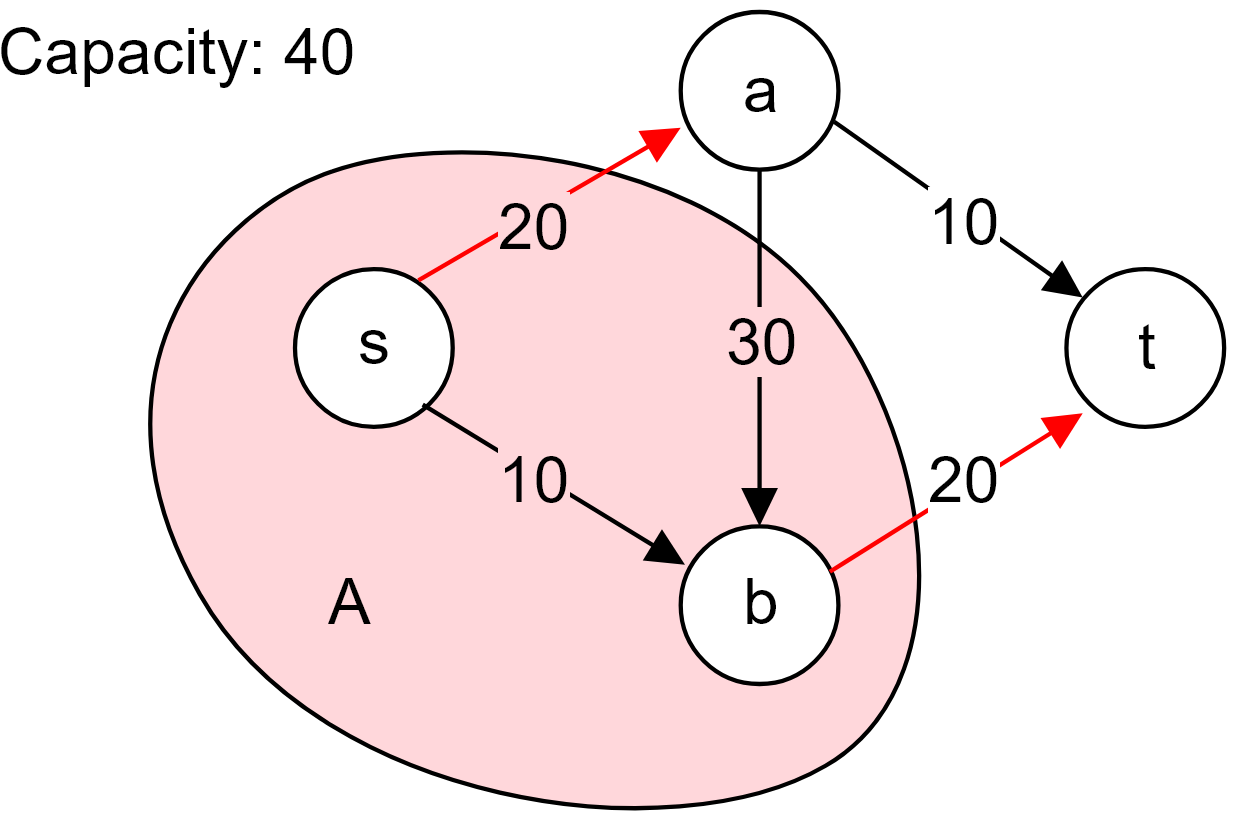
\includegraphics[width=0.5\textwidth]{Sections/net/cap.png}
        \caption{Flow Network with Capacity Cut $A$}
    \end{figure}

\noindent
Here the sum of the edge weights leaving $A$ is $c(s,a) + c(b,t) = 20 + 20 = 40$.

\begin{Def}[Minimum Cut (Min Cut)]

    A cut $C(A,B)$ such that the capacity obtained is the minimum possible value for all cuts in the graph.
\end{Def}

\begin{figure}[h]
    \centering
    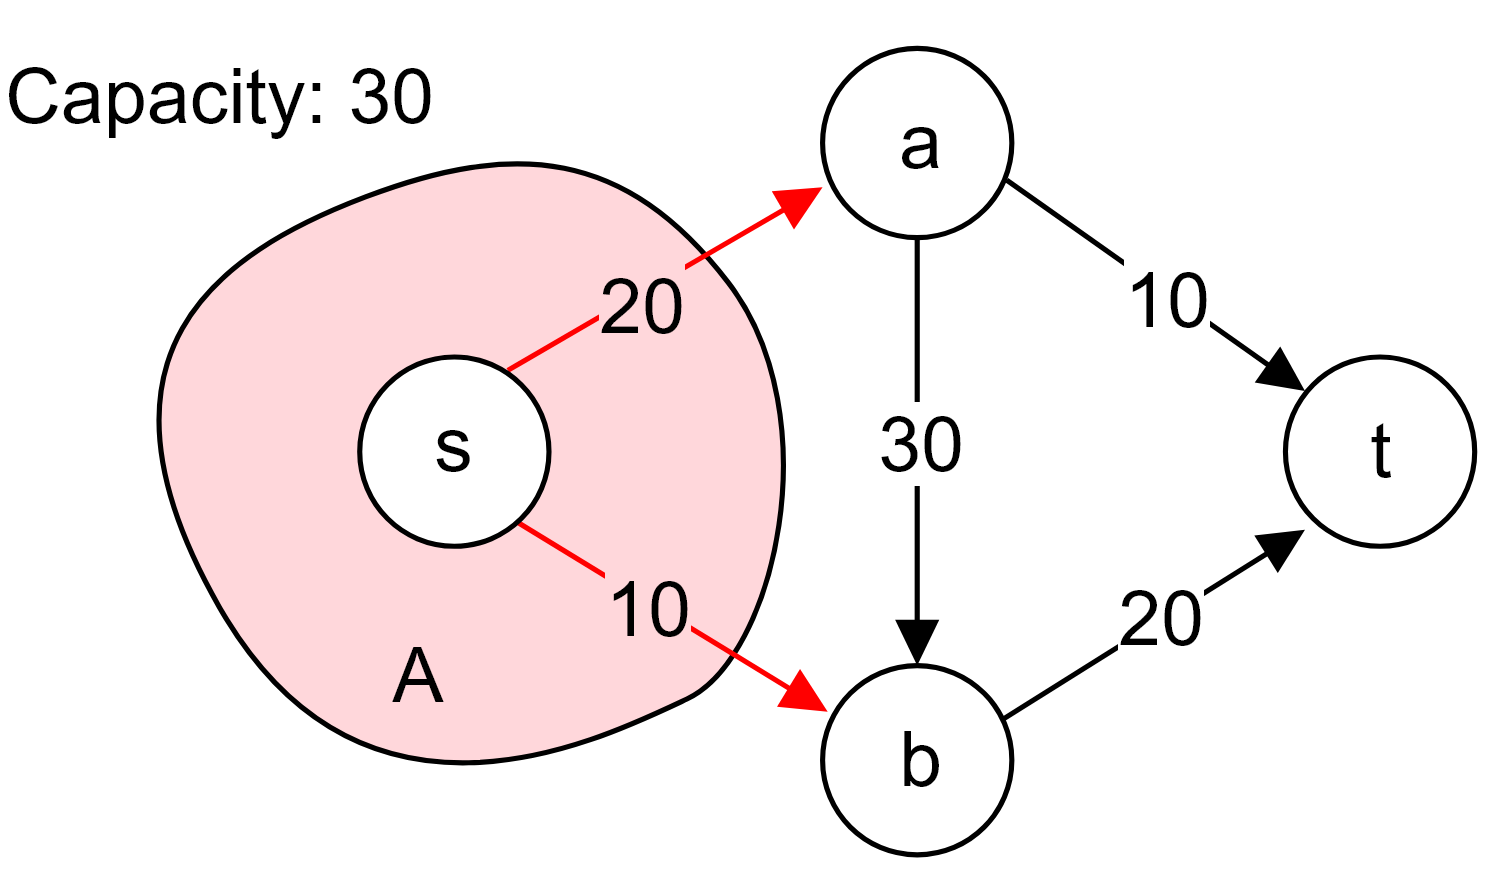
\includegraphics[width=0.5\textwidth]{Sections/net/min.png}
    \caption{Flow Network with Minimum Cut}
\end{figure}

\noindent
Where the minimum cut is $C(A,B) = 20$, as $c(s,a) + c(s,b) = 10 + 20 = 30$. Note, despite
this cut being around the source node, not all minimum cuts result in this manner.

\newpage

\begin{Def}[Graph Flow]

    For edges $(u,v)$ in a graph $G=(V,E)$, the flow $f(u,v)$ denotes the amount of data flowing from $u$ to $v$.
    For a valid \textbf{s-t flow}, $f$ in $G$ follows the following constraints:
    \begin{enumerate}
        \item [(i)] Capacity constraint: for all $(u,v)\in G$, $0 \leq f(u,v) \leq c(u,v)$ 
        \item  [(ii)] Flow conservation: for all $v \in V \setminus \{s,t\}$, ${\displaystyle \sum_{u\to v \in V} f(u,v) = \sum_{v\to w \in V} f(v,w)}$
    \end{enumerate}

    \noindent
    I.e., (i) data flows within capacity limits, and (ii) data isn't created or destroyed in the network.
\end{Def}

\vspace{-1em}
\begin{figure}[h]
    \centering
    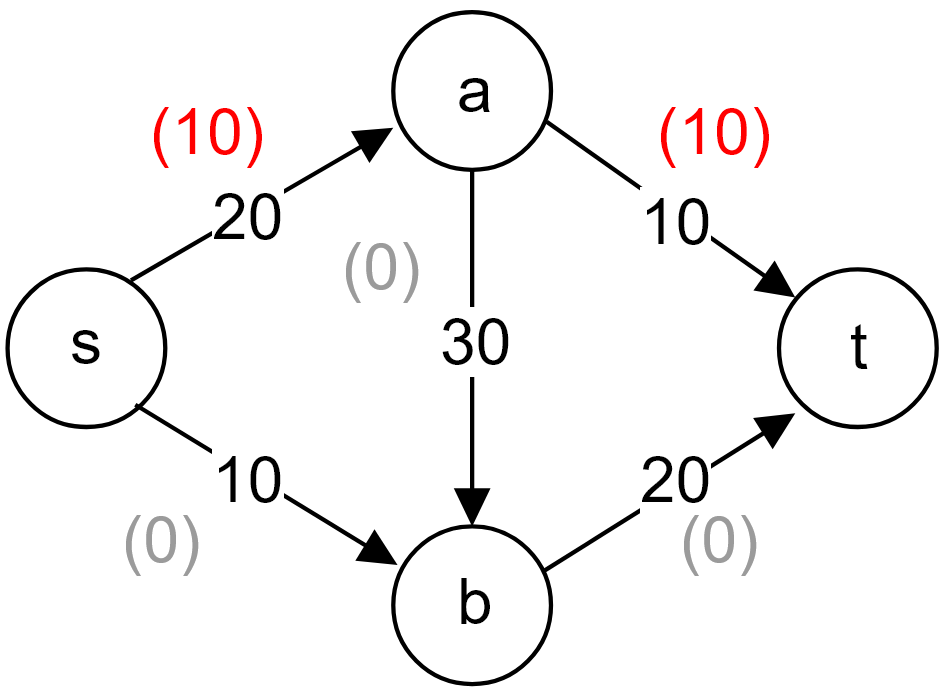
\includegraphics[width=0.35\textwidth]{Sections/net/flow.png}
    \caption{Flow Network with Flow a valid flow $f$, as what comes in, is what comes out.}
\end{figure}
\begin{Def}[Maximum Flow (Max Flow)]

    The maximum flow in a network is the maximum amount of data that can be sent from the source to the sink.
    \textbf{Integral Flow,} is a flow where all edge flows are whole integers.
\end{Def}

\begin{figure}[h]
    \centering
    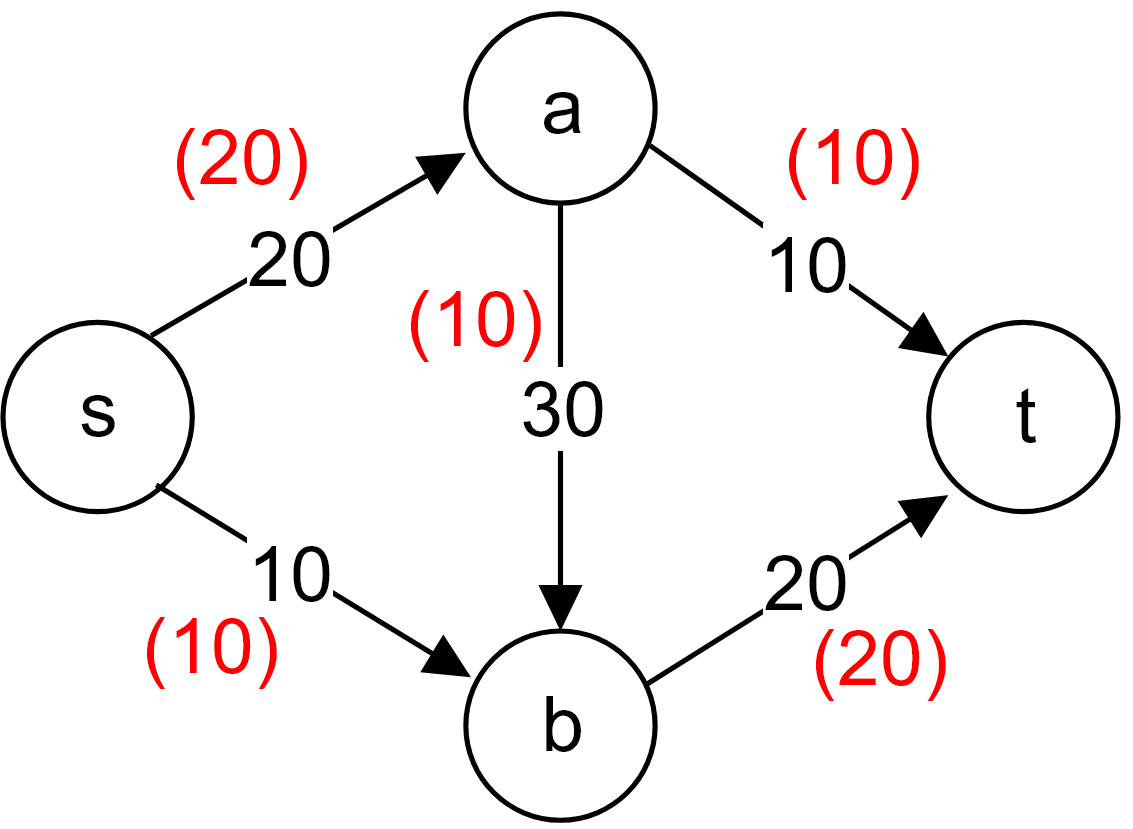
\includegraphics[width=0.35\textwidth]{Sections/net/max.png}
    \caption{Flow Network with Maximum Flow}
\end{figure}

\newpage
\begin{Def}[Flow Value Lemma]

    For any flow $f$ the value $V(f)$ and any s-t cut $C(A,B)$, the net-flow sent across the cut is equal to the flow leaving $s$, i.e.,
    for $u \in A$ and $v \in B$:
    \begin{equation}
        V(f) = \sum_{\{u\to v\}} f(u,v) - \hspace{-1em} \sum_{\{u\leftarrow v\}} f(v,u)
    \end{equation}
    Subtracting flows entering preserves conservation, as what comes in, is sent out.
\end{Def}

\begin{figure}[h]
    \centering
    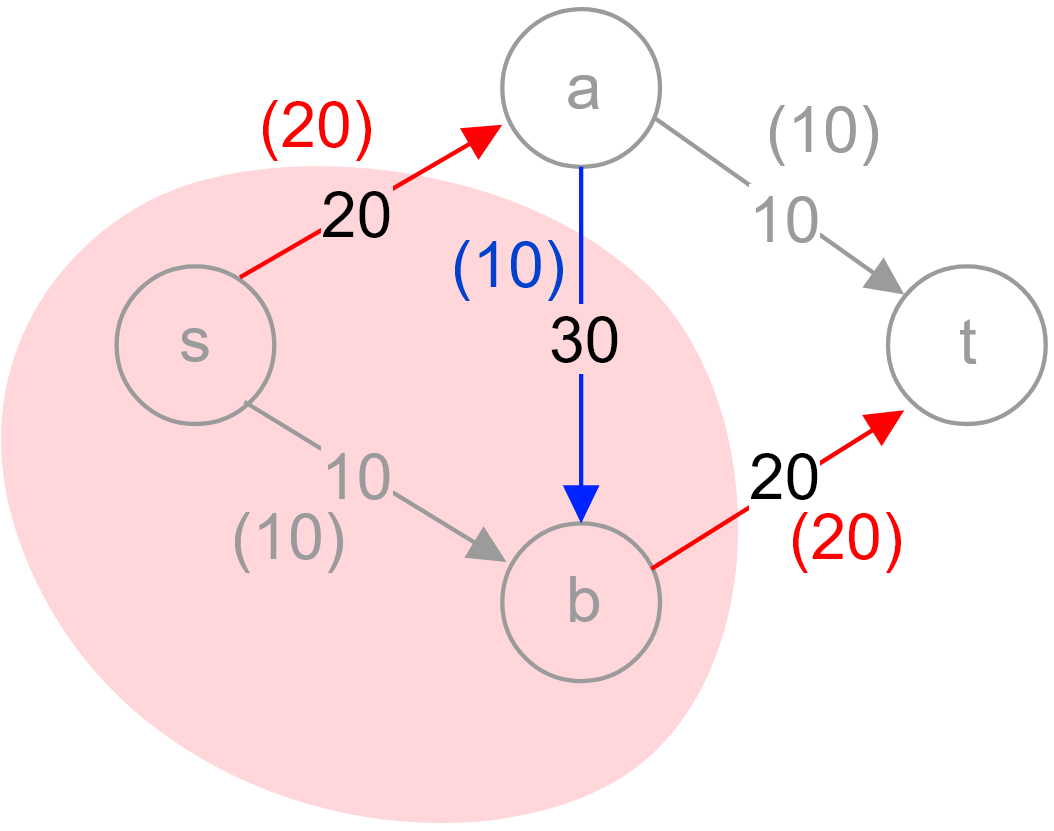
\includegraphics[width=0.35\textwidth]{Sections/net/flowval.png}
    \caption{An s-t cut with net-flow equaling $V(f)$: $(20+20)-(10) = 30 = V(f)$.}
\end{figure}

\begin{Def}[Weak Duality]

    For any flow $f$ and any s-t cut $C(A,B)$, the value of the flow is at most the capacity of the cut, i.e.,
    \begin{equation}
        V(f) \leq C(A,B)
    \end{equation}
\end{Def}

\begin{Def}[Max Flow-Min Cut Theorem]

    By weak duality, \underline{if $V(f)=C(A,B)$ then $f$ is the max-flow and $C(A,B)$ the min-cut.} As by 
    conservation, $V(f)$ cannot get any larger. If $C(A,B)$ weren't the min cut,
    $V(f)<C(A,B)$ bottle-necked by some other smaller capacity.
\end{Def}

\noindent
One could approach this problem iteratively by \textbf{augmenting} the graph by picking the largest path and 
bottle-necking the flow via the lowest capacity edge.\\

\noindent
Though the biggest problem with this approach is that, how do we consider all possible paths? We
could use recursion finding. However, this could lead to an inefficiencies or even infinite loops.

\newpage
\noindent
When filling out our graph, we may want to keep track of what choices we made, and how much flow we have left to give.
For this we introduce the following data structure:
\begin{Def}[Residual Graph]

    Given a graph $G=(V,E)$ with flow $f$, we denote its residual graph $G_f = (V,E_f)$, where $E_f$ are a new set of edges generated from augmentations.
    Between two nodes $u$ and $v$ in $G_f$, we have the following edges:
    \begin{itemize}
        \item Flow spent from $u$ to $v$, $f(u,v)$, is shown as a \textbf{backward edge} $c_b$ of that capacity, $$c_b(u,v):= f(u,v)$$.
        
        \vspace{-2em}
        \item Flow left to spend is shown as a \textbf{forward edge} $c_f$ with capacity of what's left, $$c_f(u,v) := c(u,v) - f(u,v)$$
    \end{itemize}

    \vspace{-1em}
\end{Def}

\vspace{-1em}
\begin{figure}[h]
    \centering
    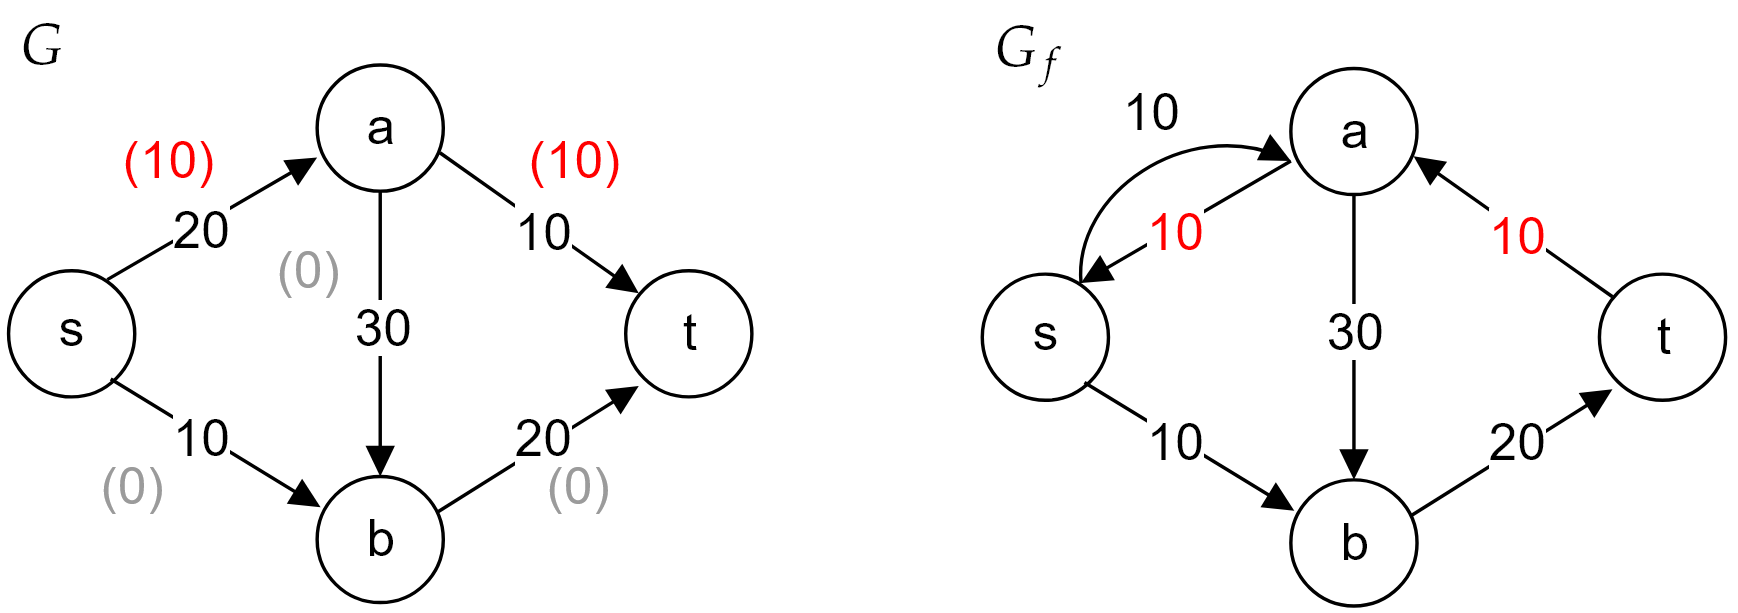
\includegraphics[width=.8\textwidth]{Sections/net/res.png}
    \caption{A graph $G$ and its residual graph $G_f$.}
\end{figure}

\noindent
Our residual graph tells us, going from $s$ to $t$, what paths we can take, and how much flow we have left to spend.
We harness this into the following algorithm:
\begin{theo}[Ford-Fulkerson Algorithm (FFA)]

    Given a flow network $G=(V,E)$, with source $s$ and sink $t$, the Ford-Fulkerson algorithm finds the max flow by iteratively augmenting the graph.
    \begin{enumerate}
        \item Initialize flow $f(u,v) = 0$ for all $(u,v) \in E$.
        \item While there exists a path $p$ from $s$ to $t$ in $G_f$, augment the flow along $p$.
        \item Return the flow $f$.
    \end{enumerate}

    \noindent
    Notably, if a backward edge $c_b(u,v)$ is taken from $s\to t$, then $f(u,v)\in G$ is decreased by $c_b(u,v)$.
    Additionally, each output is an integral flow.
\end{theo}
\newpage 

\noindent
In essence, each round we find a path from $s\to t$ in $G_f$, take that path and update both tables $G$ and $G_f$ with the new flow. Do 
so until we no longer can reach $t$ from $s$ in $G_f$.

\begin{figure}[h]
    \centering
    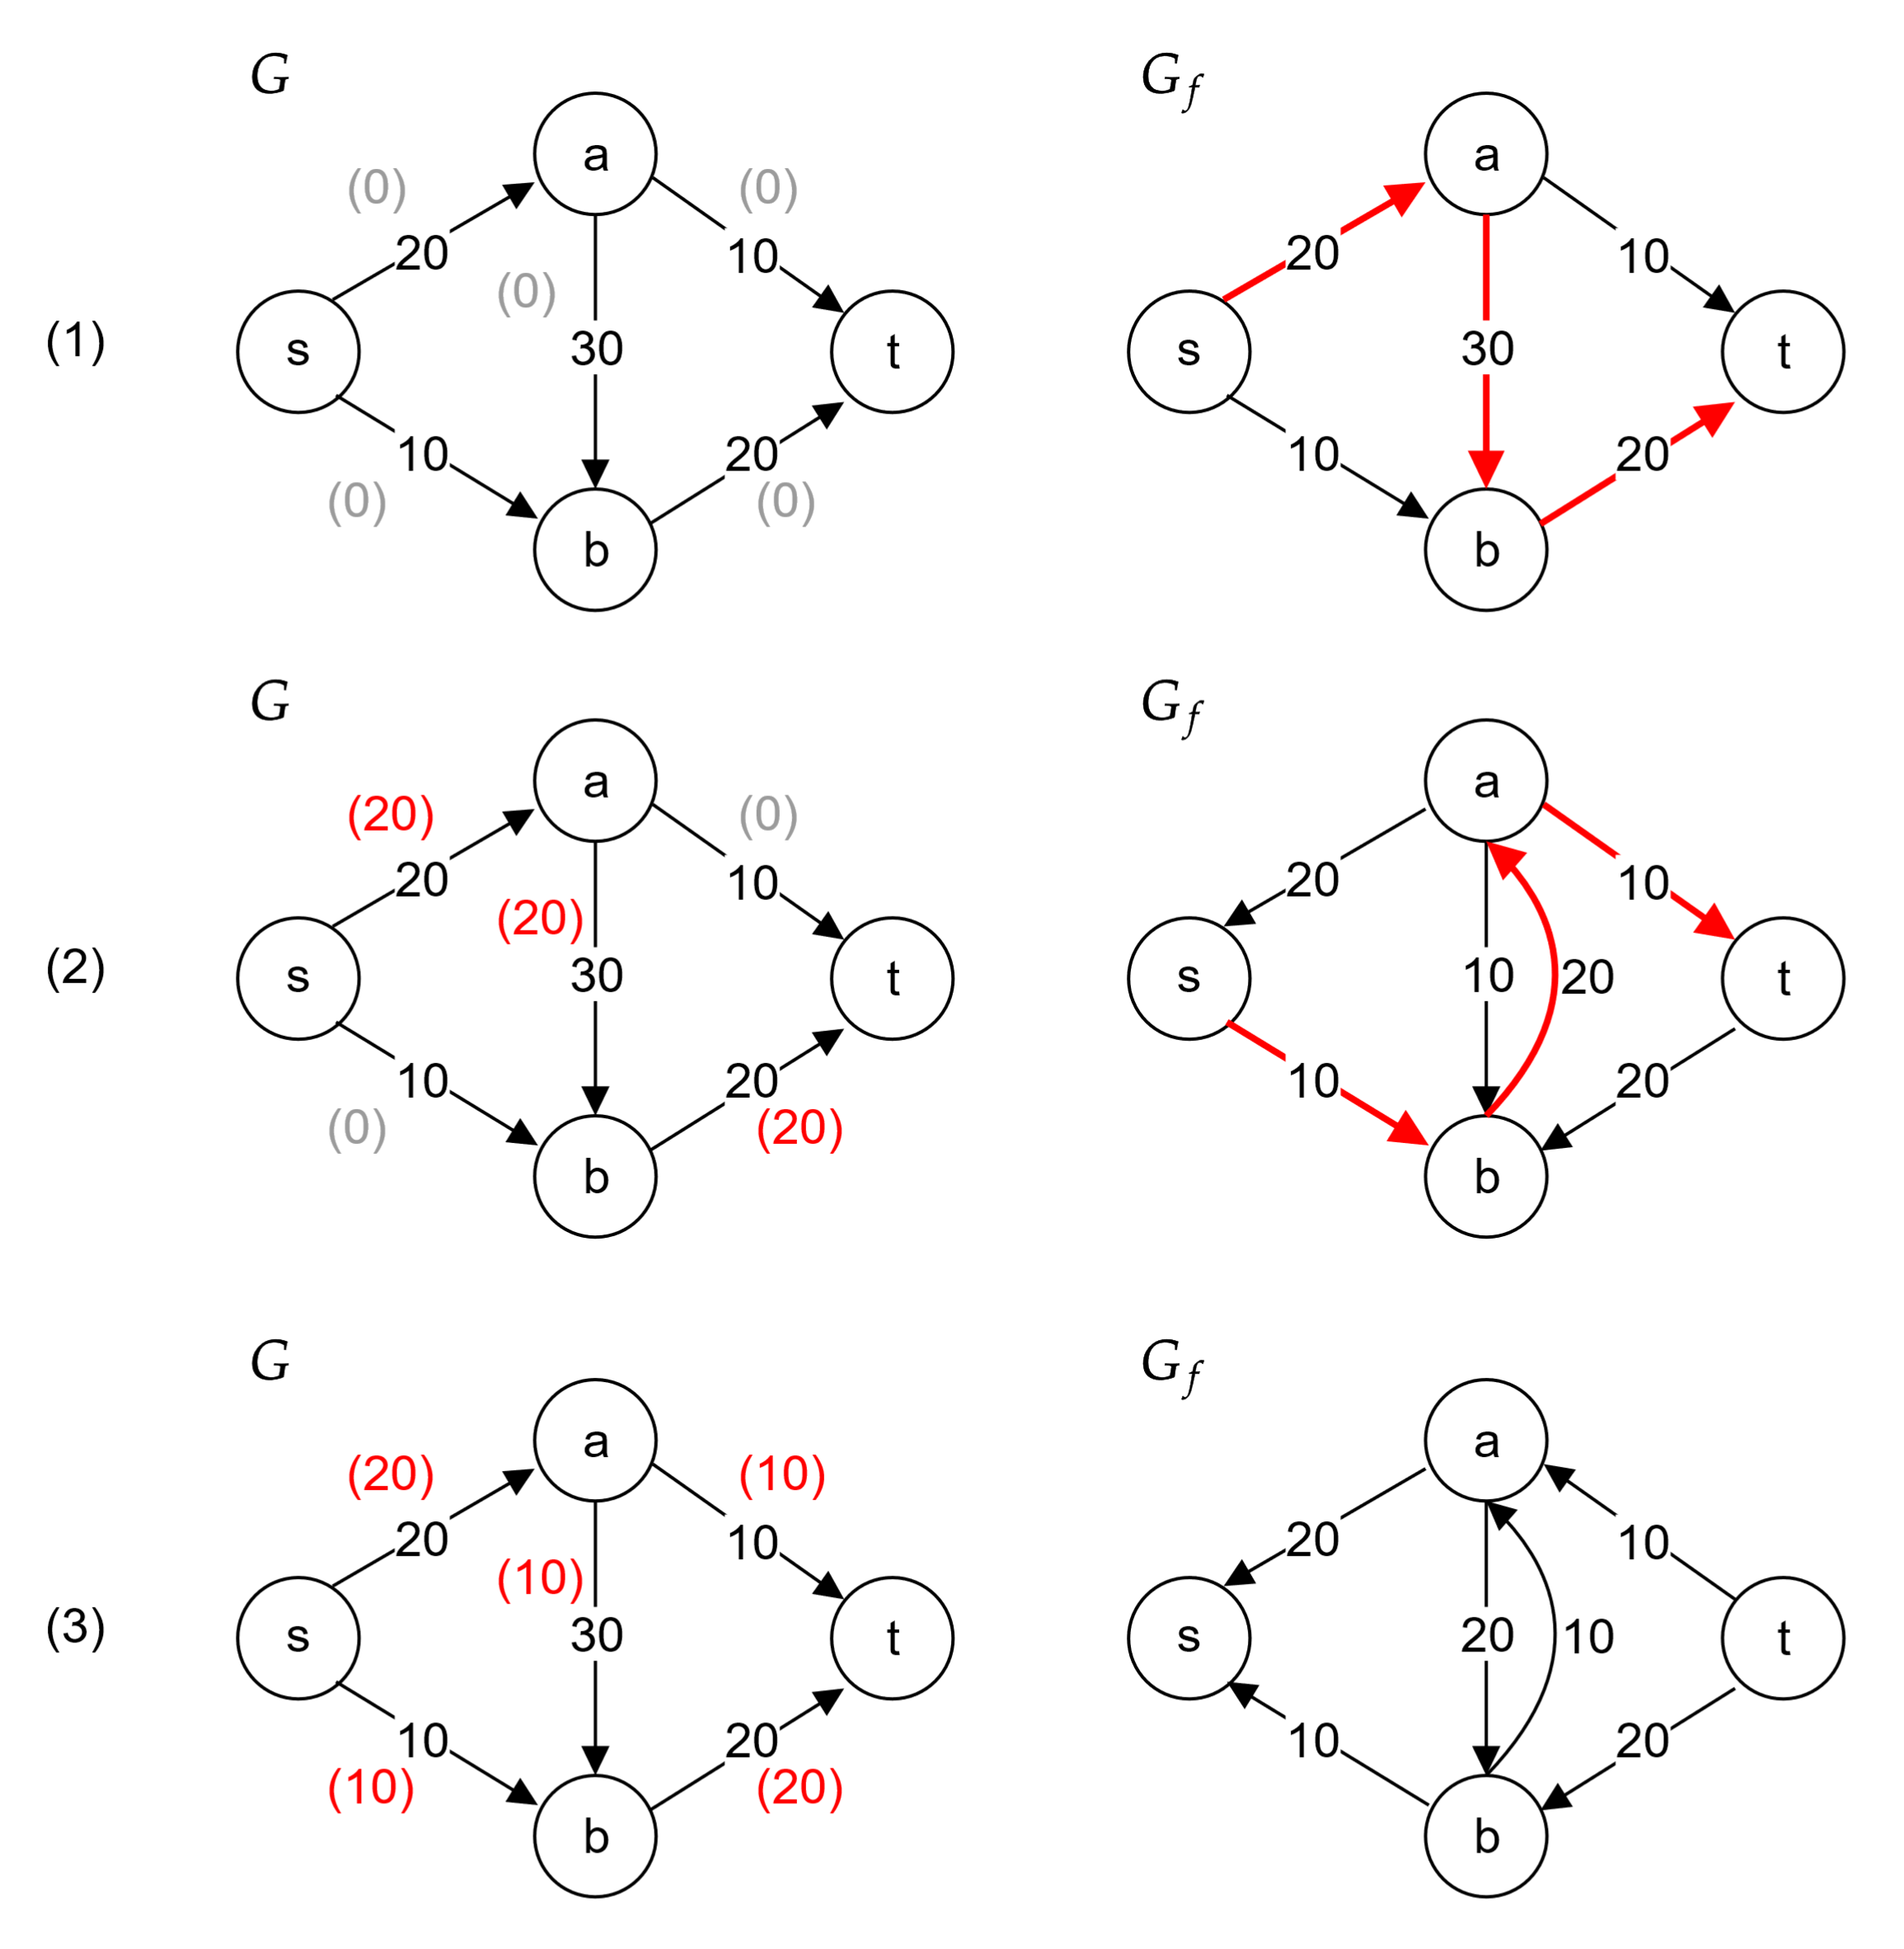
\includegraphics[width=.8\textwidth]{Sections/net/ff.png}
    \caption{Ford-Fulkerson Algorithm in action, terminating at 3 where $s\to t$ is blocked.}
\end{figure}

\begin{theo}[Ford-Fulkerson Max flow-Min Cut Consequence]

    At termination, max flow is obtained. Moreover, nodes from $s$ to blocked nodes $b$ form a cut $C(A,B)$, which is the min cut.
\end{theo}

\vfill

\begin{center}
    \textit{Algorithm on next page.}
\end{center}

\vfill

\newpage

\begin{Func}[Ford-Fulkerson - \textit{Ford-Fulkerson($G, s, t, c$)}]

    \vspace{-.5em}
    \begin{algorithm}[H]
        \SetKwProg{Fn}{Function}{:}{}
        \KwIn{$G$: graph, $s$: source, $t$: sink, $c$: capacities}
        \KwOut{$f$: maximum flow}

        \vspace{.5em}
        \Fn{\textit{Ford-Fulkerson($G, s, t$)}}{

            \vspace{.5em}
            \ForEach{$e \in E$}{
            $f(e) \gets 0$ \tcp{Initialize flow on each edge to zero}
            }

            \vspace{.5em}
            $G_f \gets \textit{residual}(G, f)$ \tcp{Construct the residual graph}

            \vspace{.5em}
            \While{there exists path $P:= s\to t$ in $G_f$}{
            $f \gets \textit{Augment}(f, P)$ \tcp{Augment the flow along path $P$}
            Update $G_f$ along $P$\;
            }

            \vspace{.5em}
            \Return $f$\;
        }
    \end{algorithm}
    
    \noindent
    \rule{\textwidth}{0.4pt}
    \textbf{Time Complexity:} $O(mnC)$, where $m$ is the number of edges, $n$ is the number of nodes, 
    and $C$ is the value of the maximum flow. Line 5 takes $O(m)$ time to find an augmenting path in the residual graph. Lines 6-7 take $O(n)$ time to update the flow along the path. Since the flow increases by at least 1 unit in each iteration, and each iteration takes $O(m + n) = O(m)$ time, the while loop runs at most $C$ times. Therefore, the total time complexity is $O(mnC)$.

\end{Func}

\begin{Func}[Augmentation for Ford-Fulkerson - \textit{Augment($f, c, P$)}]

    \vspace{-.5em}
    \begin{algorithm}[H]
        \SetKwProg{Fn}{Function}{:}{}
        \KwIn{$f$: current flow, $c$: capacities, $P$: augmenting path}
        \KwOut{$f$: updated flow}

        \vspace{.5em}
        \Fn{\textit{Augment($f, P$)}}{
            $b \gets \textit{bottleneck}(P)$ \tcp{Minimum residual capacity of an edge in $P$}
                
            \ForEach{$e \in P$}{
                \uIf{$e \in E$}{
                    $f(e) \gets f(e) + b$ \tcp{Update flow on forward edge}
                }
                \Else{
                    $f(e) \gets f(e) - b$ \tcp{Update flow on reverse edge}
                }
            }
            \Return $f$\;
        }
    \end{algorithm}
    
    \noindent
    \rule{\textwidth}{0.4pt}
    \textbf{Time Complexity:} $O(n)$, where $n$ is the number of nodes in $G$. At worst our path $P$ contains all nodes.
\end{Func}

\newpage 

\begin{theo}[Residual Graph Min-cut Corollary]
    
        Given a network-flow that has reached its max-flow, a min cut can be found in one of two ways using an s-t cut $C(A,B)$:
        \begin{itemize}
            \item \textbf{From s}: Let $A$ be the partition of nodes reachable from $s$ in the residual graph. Then the cut formed by a is a min cut.
            \item \textbf{To t}: Let $B$ be the partition of nodes that reach $t$ in the residual graph. Then the cut formed by $B$ is a min cut.
        \end{itemize}
\end{theo}
\begin{figure}[h!]
    \centering
    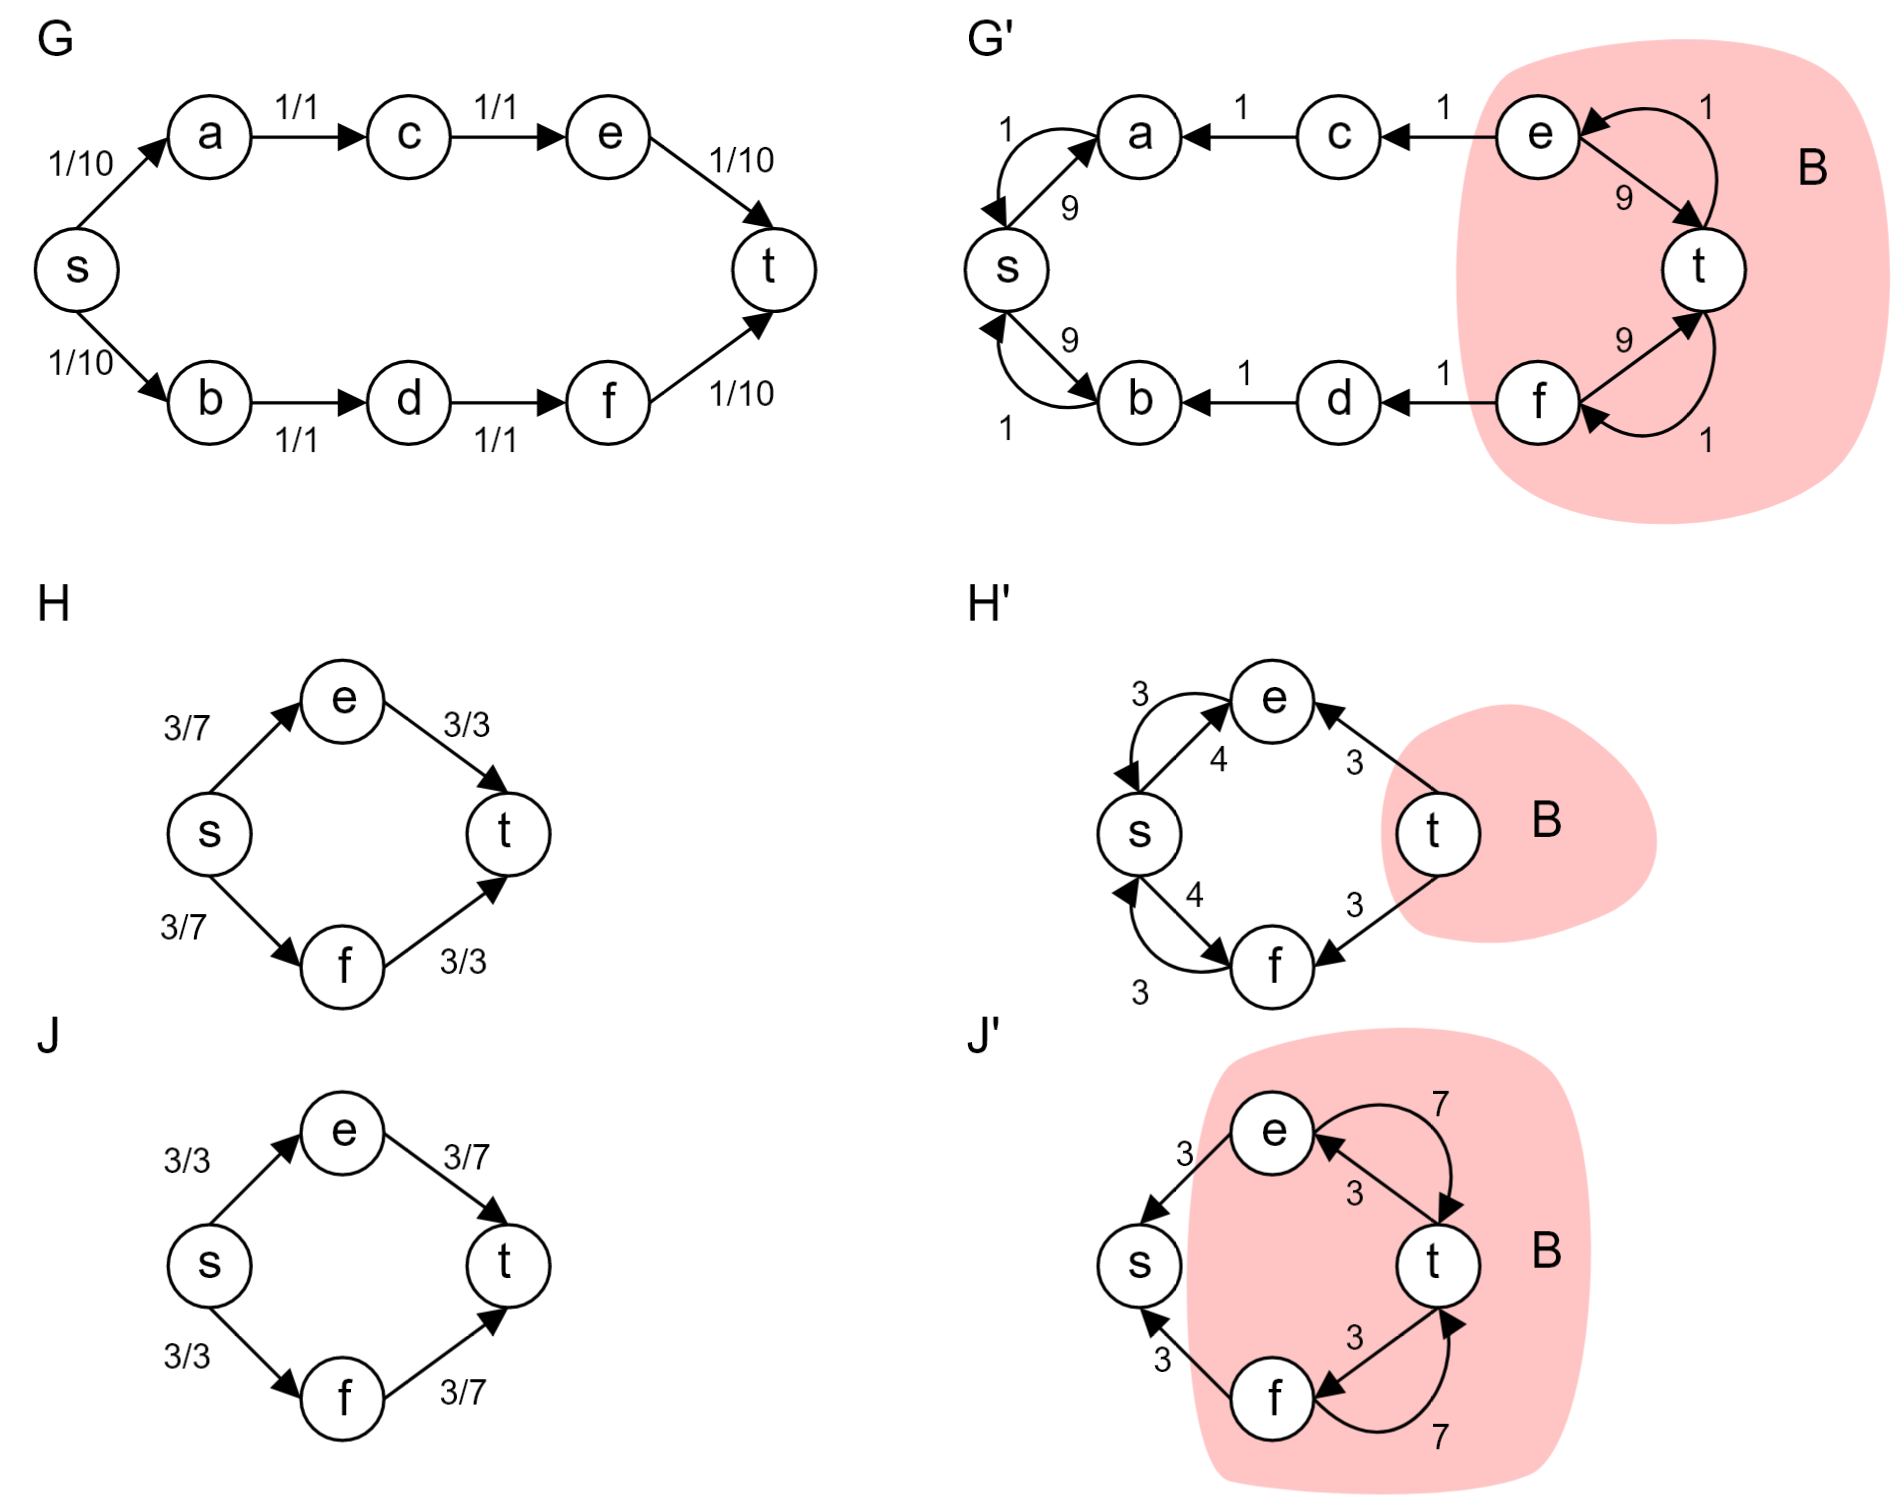
\includegraphics[width=1\textwidth]{Sections/net/tot.png}
    \caption{Network flows graphs adjacent to their residual graphs showing min-cut partitions.}
    \label{fig:tot}
\end{figure}

\noindent
The above graph shows examples of $C(A,B)$ cuts forming min-cuts by nodes in $B$ reaching the sink $t$ in the residual graph.

\newpage
\section{Bipartite Matching}
In this section we revisit matching problems alike what we saw with Gale-Shapely, Section (\ref{sec:stable-match}). Here we find
the maximum number of matches between two sets of elements, $L$ and $R$, where each element from both sets may partially match some 
set of elements from the other.
\begin{Def}[Bipartite Graph]

    Given a graph $G=(V, E)$, such that $V:=L\cup R$, where $E$ connects nodes $L$ to $R$,
    a cut which separates $V$ into the two sets $L$ and $R$ is called a \textbf{Bipartition}. 
\end{Def}

\vspace{-.5em}
\begin{figure}[h]
    \centering
    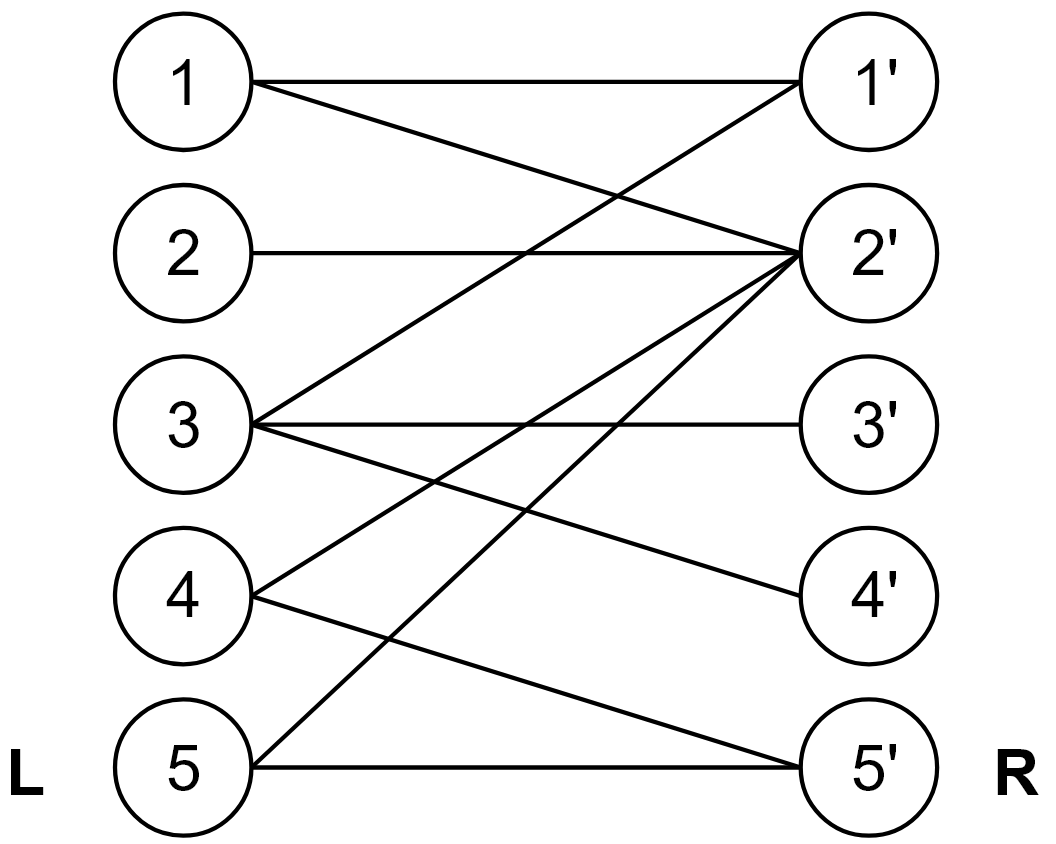
\includegraphics[width=.35\textwidth]{Sections/net/bip.png}
    \caption{A Bipartite Graph $G(V,E)$ cut into two sets $L:=\{1,\dots,5\}$ and $R:=\{1',\dots,5'\}$.}
    \label{fig:bip}
\end{figure}

\noindent
Think, if we had water flowing from $L$ to $R$, what maximum-flow would arise, how many networks could we utilize?

\begin{figure}[h]
    \centering
    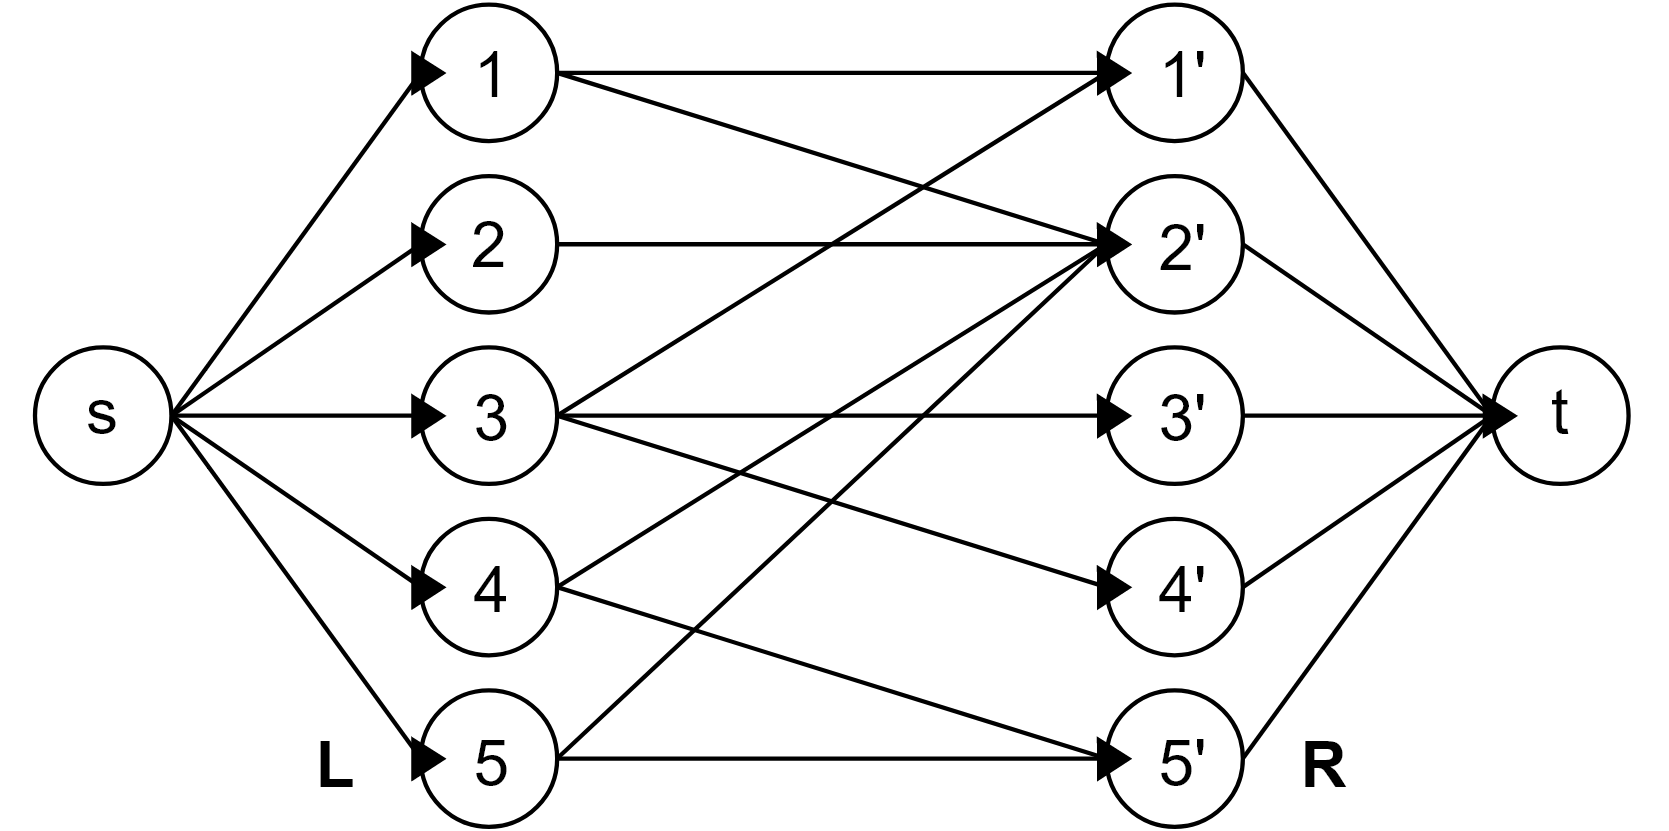
\includegraphics[width=.5\textwidth]{Sections/net/bipflow.png}
    \caption{Figure (\ref{fig:bip}) with a source node $s$ added to $L$ and sink $t$ added to $R$.}
\end{figure}

\noindent
\begin{theo}[Max-Matching \& Max-Flow]

    Given a bipartite graph $G=(L\cup R,E)$ with a source and sink from $L\to R$, the flow which runs through nodes $L\to R$ is the maximum matching, each edge a capacity of 1.  
\end{theo}

\newpage 
\noindent

The below diagram demonstrates a maximum matching achieved through a max-flow algorithm.

\begin{figure}[h]
    \centering
    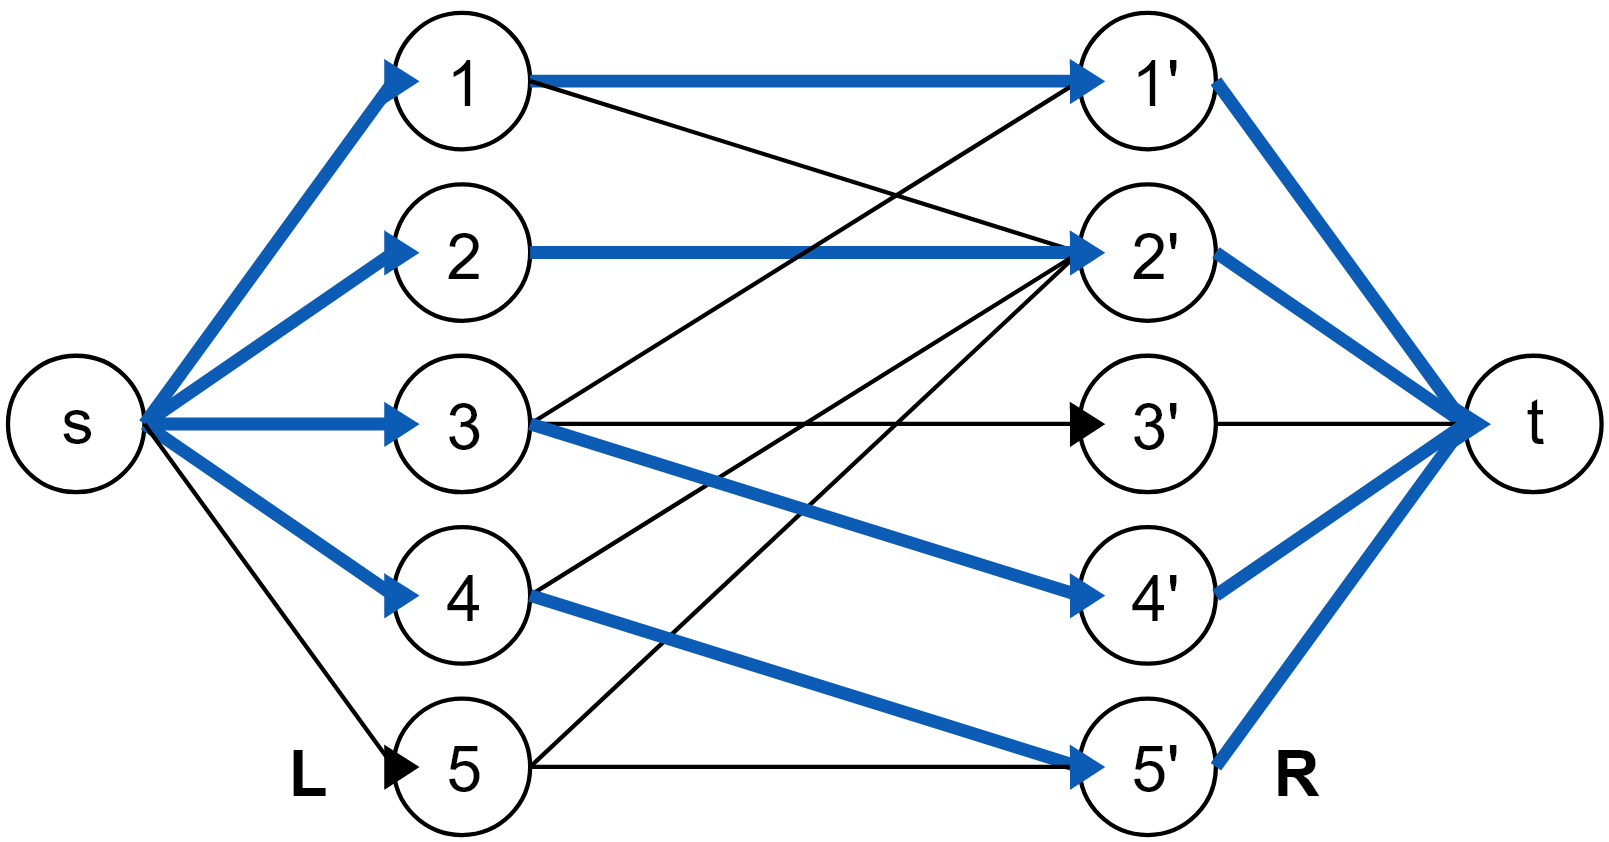
\includegraphics[width=.45\textwidth]{Sections/net/bipmax.png}
    \caption{A maximum matching found through max-flow.}
\end{figure}

\vspace{-1.5em}
\section{Edge-disjoint Paths}
\begin{Def}[Edge-disjoint Paths]

    Given a graph $G=(V,E)$, two paths $p_1$ and $p_2$ are edge-disjoint if they share no edges in common. Though, 
    they may share nodes.
\end{Def}

\vspace{-.5em}
\begin{figure}[h]
    \centering
    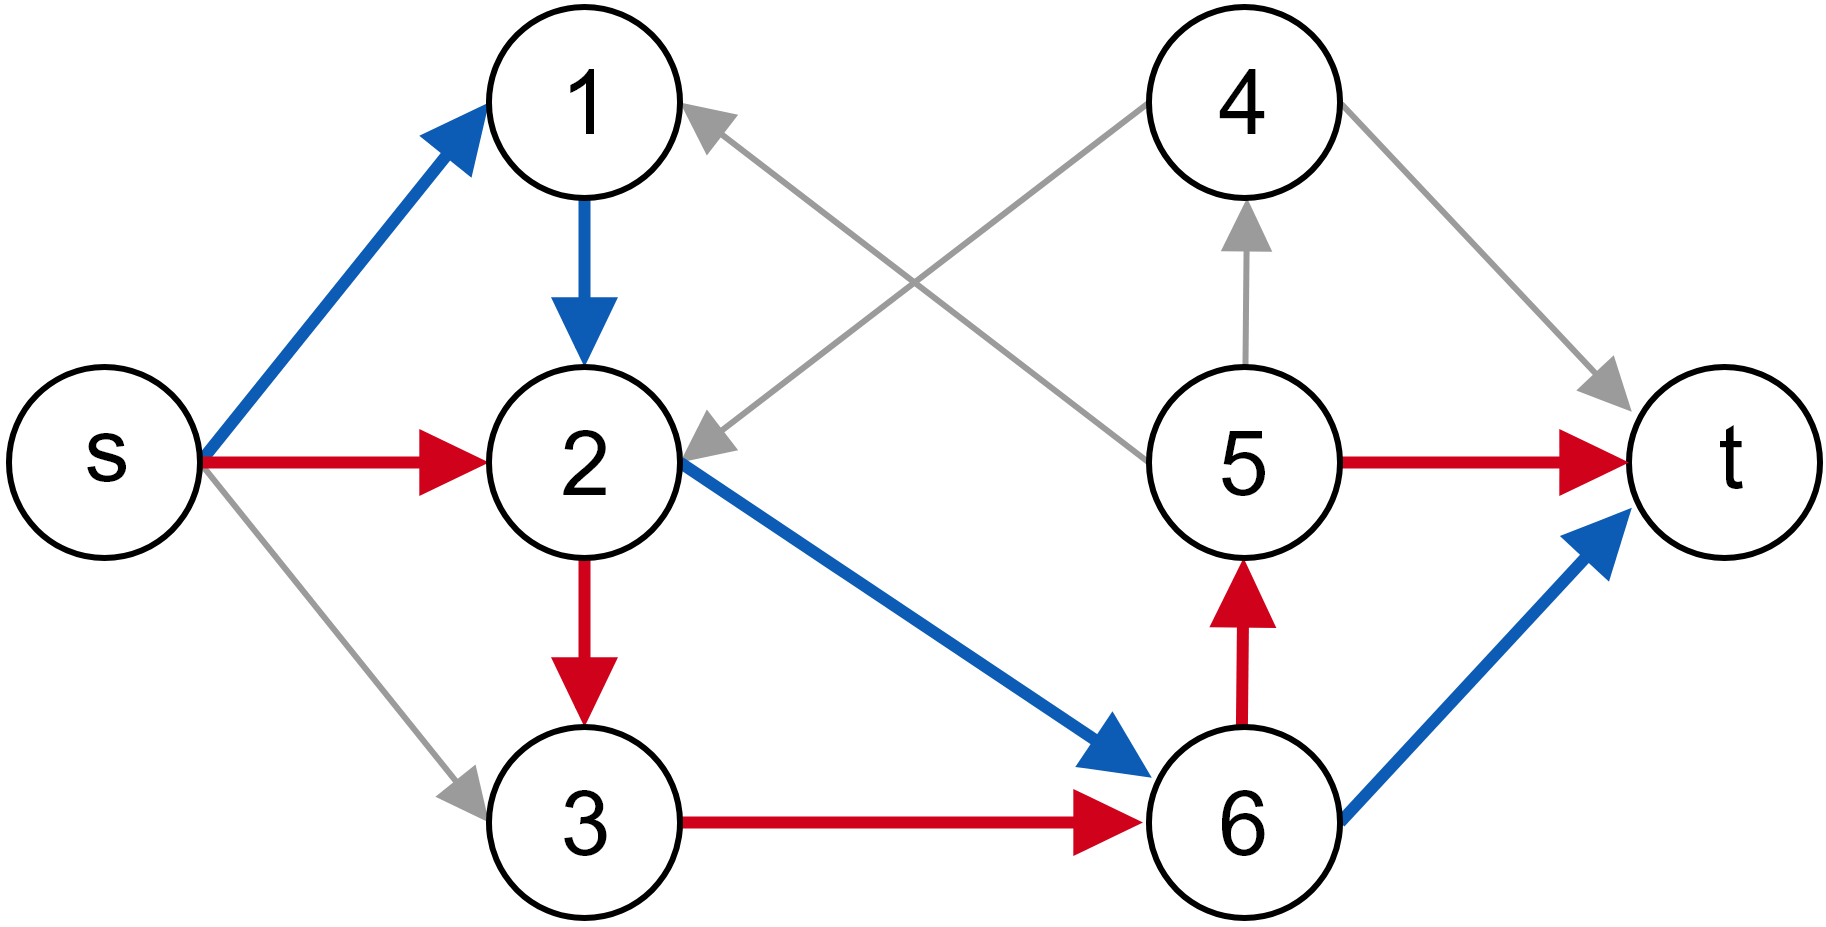
\includegraphics[width=.4\textwidth]{Sections/net/dis.png}
    \caption{Two edge-disjoint paths $p_1$(\textcolor{red}{red}) and $p_2$(\textcolor{blue}{blue}) from $s$ to $t$.}
    \label{fig:dis}
\end{figure}

\vspace{-.5em}
\begin{theo}[Max-Edge Disjoint Paths]

    The max-number of edge-disjoint paths from sink to source is the max-flow.
\end{theo}

\vspace{-1em}
\begin{figure}[h]
    \centering
    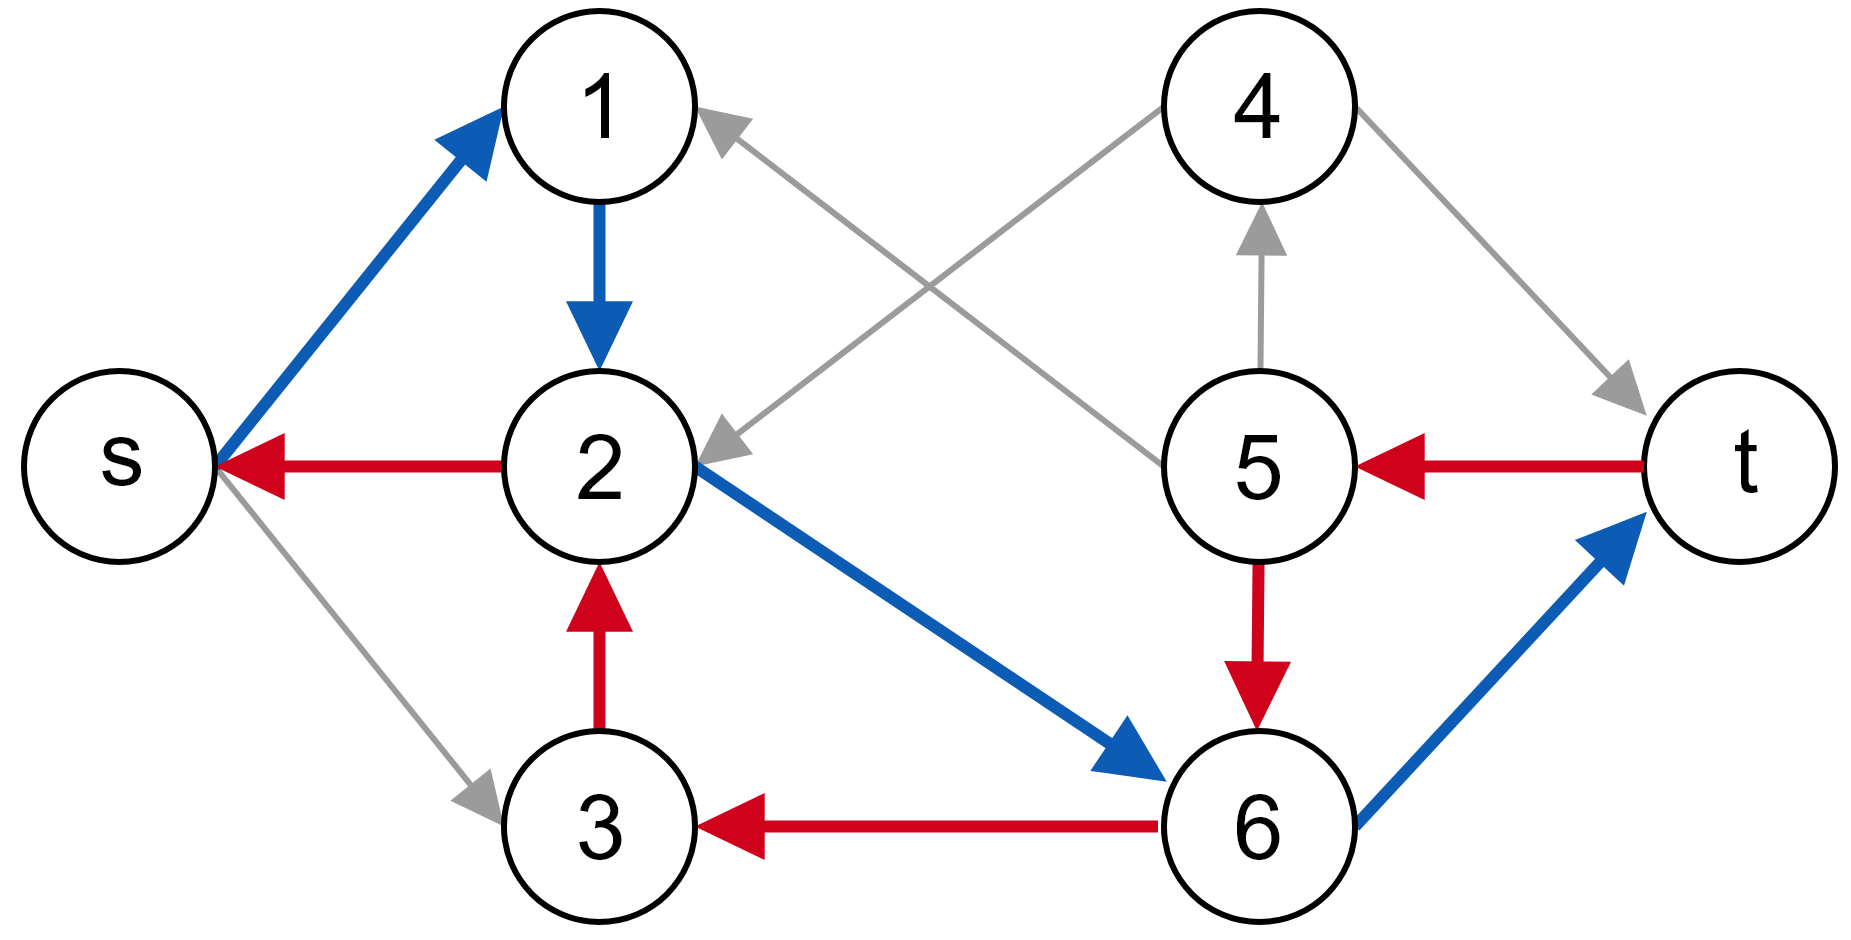
\includegraphics[width=.4\textwidth]{Sections/net/resdis.png}
    \caption{Figure (\ref{fig:dis}) of flow 2, now of flow 1 after deleting $p_1(\textcolor{red}{red})$.}
\end{figure}

\noindent
Deleting a path subtracts 1 from the flow. Hence, the number of unique paths equates to max-flow.
\newpage 
\section{Multiple Sources \& Sinks}
\textbf{Scenario - \textit{Farmer's Dilemma}:} There are multiple $c$ communities in the area
which require $x$ number of resources, and $f$ farmers. The farmers need know with the routes they have,
are they meeting community needs?

\begin{figure}[h]
    \centering
    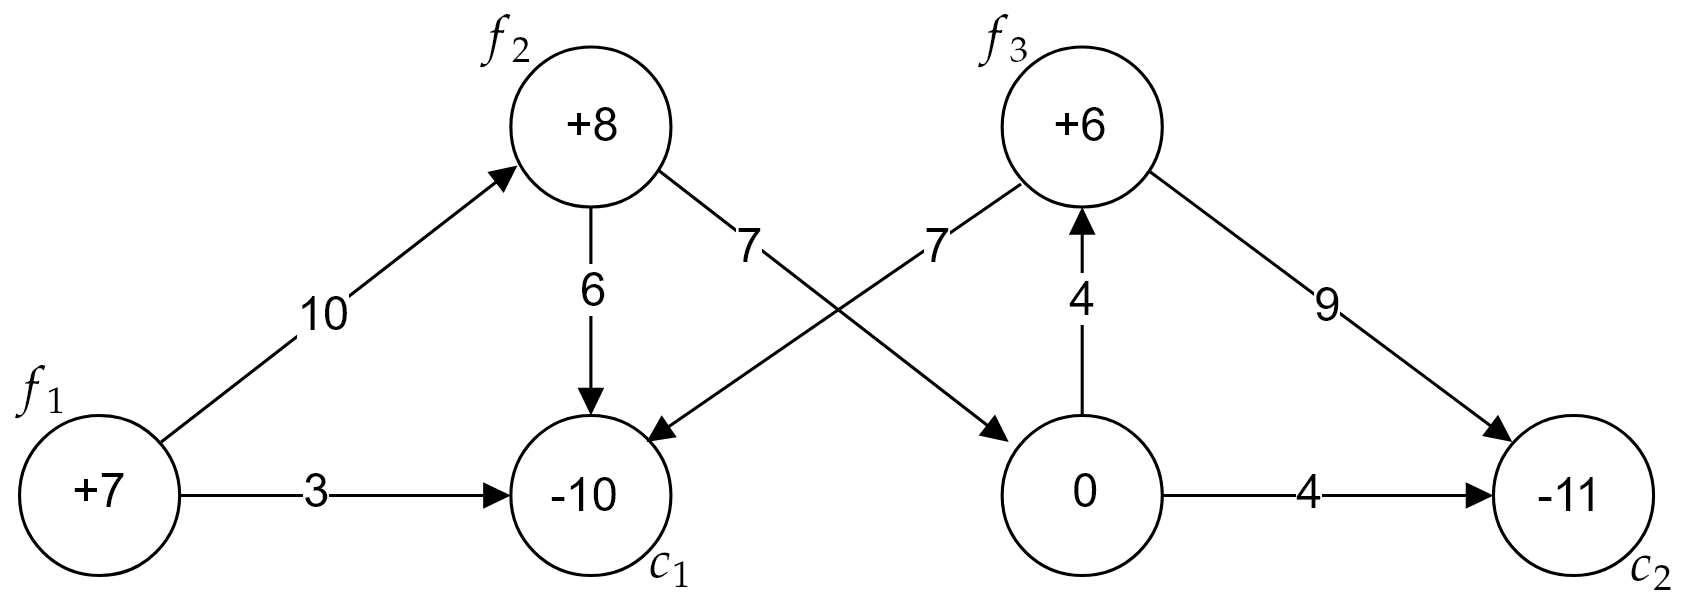
\includegraphics[width=.6\textwidth]{Sections/net/farm.png}
    \caption{A graph showing $f_j$ farms' variation connections to $c_k$ communities. (+) denoting the amount of 
    resources added and (-) the amount of resources taken.}
    \label{fig:farm}
\end{figure}

\begin{Def}[Super Source \& Sink]

    Given a graph $G=(V,E)$, with multiple sources $s_1,\dots,s_f$ and sinks $t_1,\dots,t_c$. A node 
    which acts as a source for all sources is called a \textbf{Super Source}, and a node which acts as a sink for all sinks, a \textbf{Super Sink}.
\end{Def}

\begin{figure}[h]
    \centering
    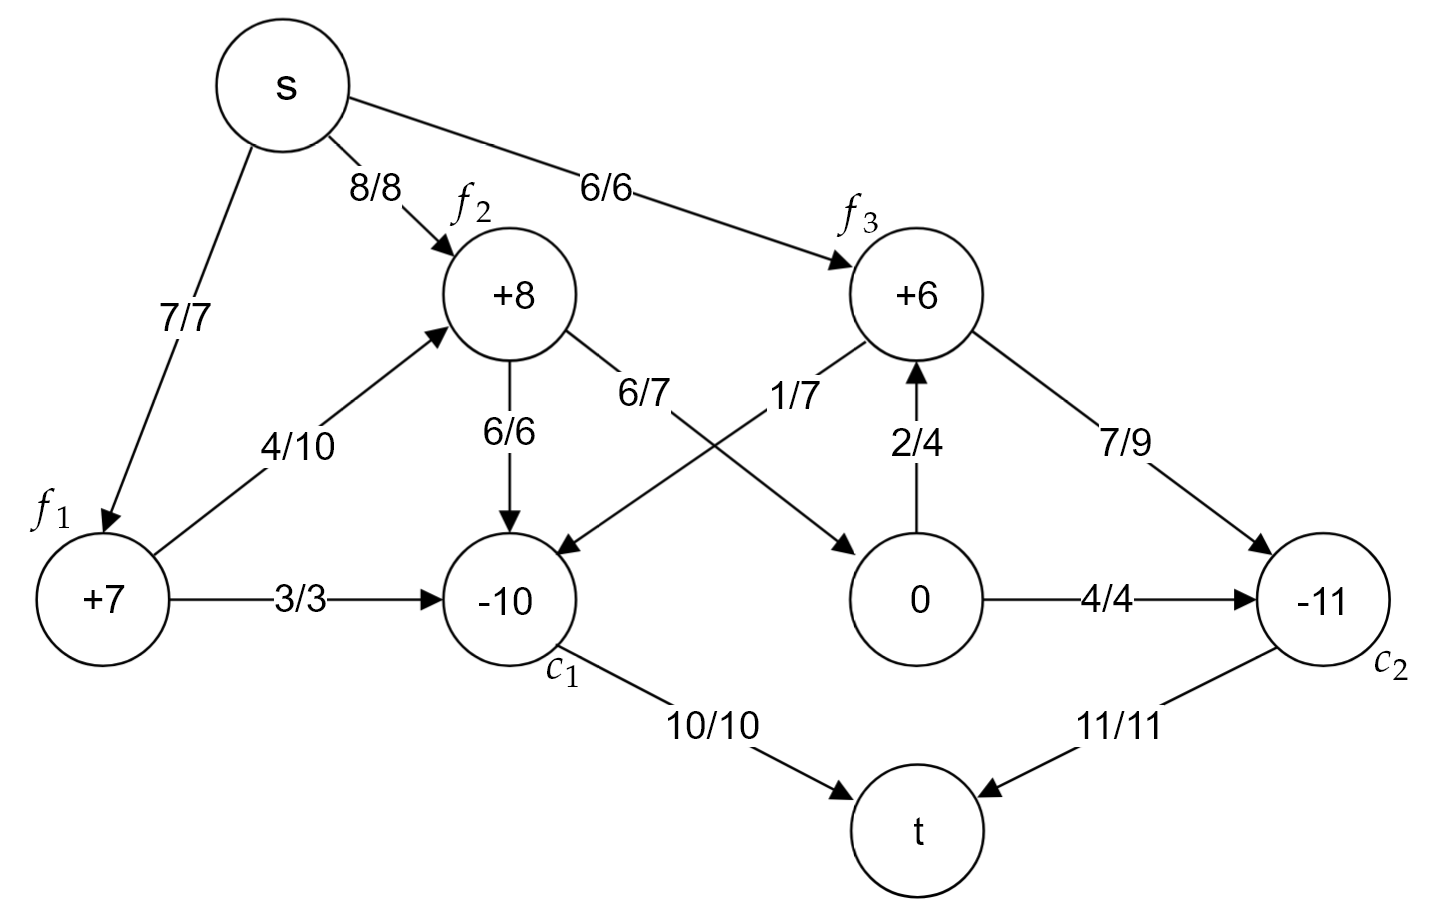
\includegraphics[width=.6\textwidth]{Sections/net/farmres.png}
    \caption{A graph with a super source $s$ and super sink $t$ on Figure (\ref{fig:farm}).}
\end{figure}

\vspace{-1em}
\noindent
Converting the graph into a flow network allows us to find the max-flow, via algorithms like Ford-Fulkerson. To verify
if demands are met, we check that the edges entering the super sink $t$ are fully saturated.\\

\noindent
The strategy is to identify a \textbf{Supply} and \textbf{Demand} relationship. If this relationship can be established, 
a bipartite graph can be formed, and a source and sink added to find the max-flow.

\newpage

\noindent
\textbf{Scenario - \textit{Eldritch Curse}:} A wizardry school needs $j$ adjunct students on 
$k$ days to help keep an Eldritch Curse sealed beneath the school. Students $W_z$, $z:=\{1,\dots,n\}$, give a list $A$ of availability on
$D_y$, $y:=\{1,\dots,m\}$ days. The school needs to know if they have enough students to keep the curse sealed for each day.\\

\noindent
We identify: \textbf{Suppliers} students $W_z$, and \textbf{demands} as days $D_y$. We now form a bipartite graph.

\begin{figure}[h]
    \centering
    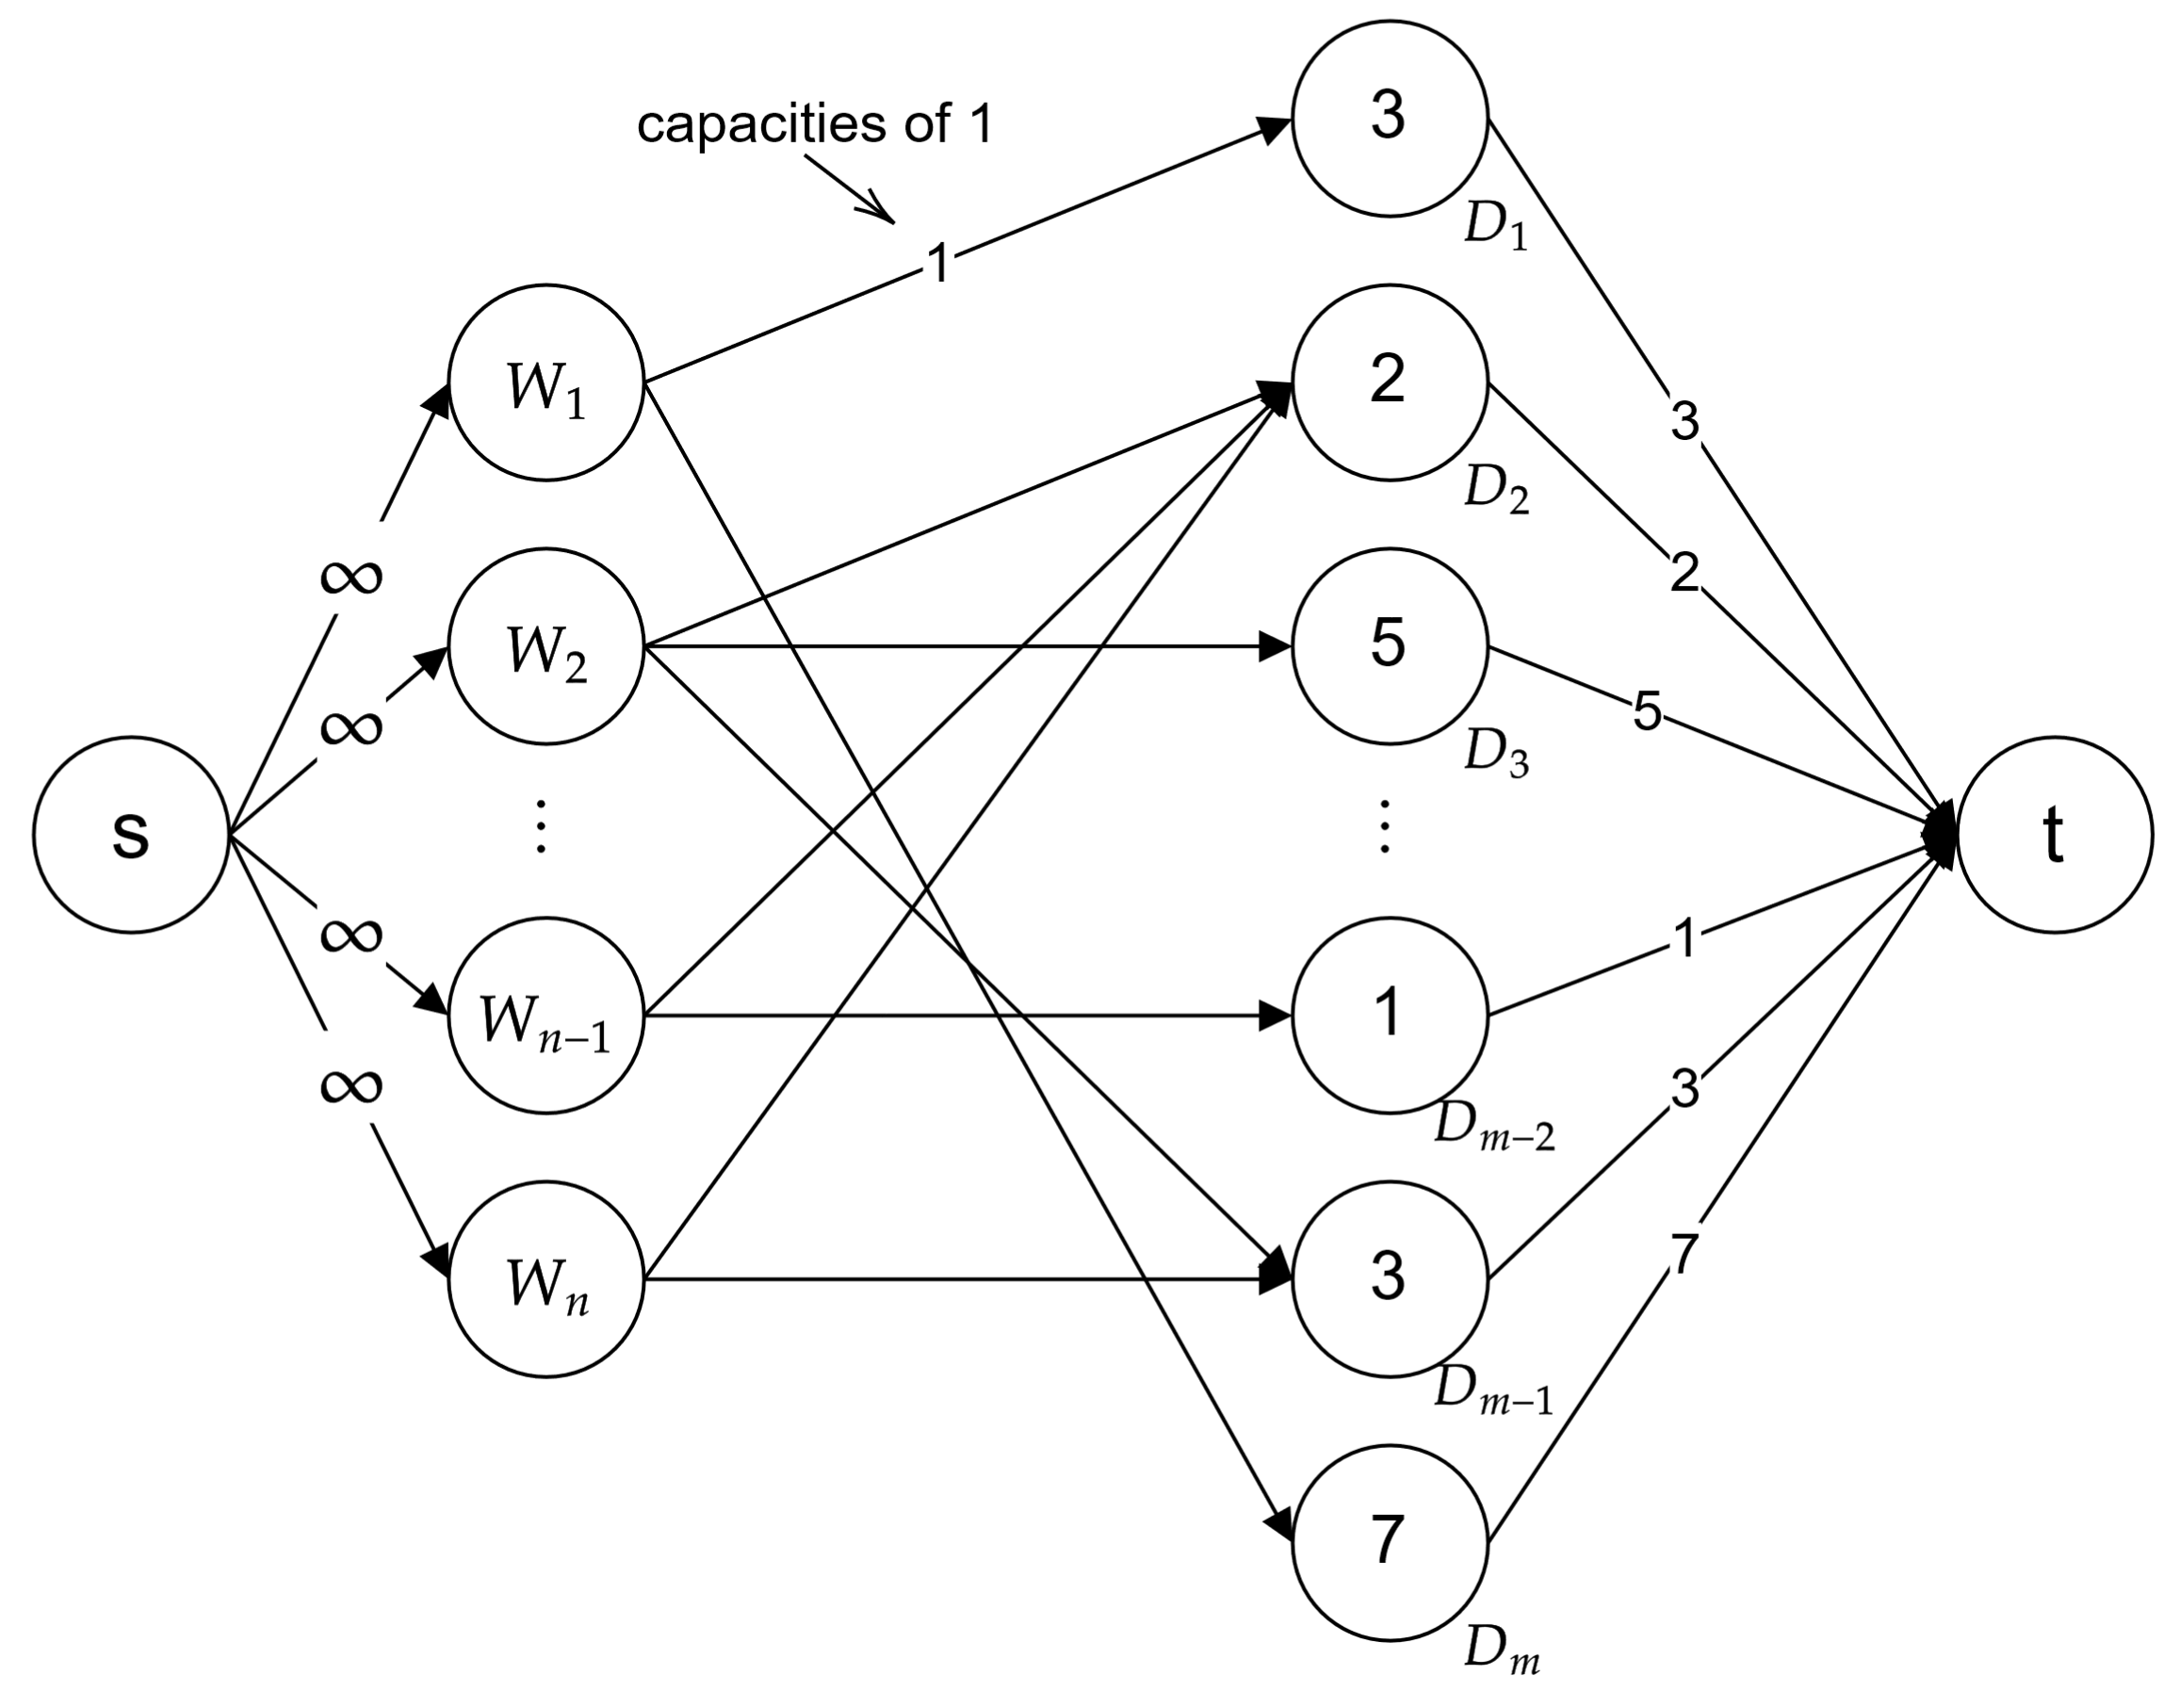
\includegraphics[width=.7\textwidth]{Sections/net/wizards.png}
    \caption{A network flow of $W_z$'s availability on $D_y$ nodes showing the students needed.}
\end{figure}

\noindent
Here the capacities leaving source node $s$ are infinite, as they will be bottleneck by the students' availability. 
We match each student to their days all with a capacity of 1. We take all capacities $C$ and flows $F$ entering the sink node $t$
and verify if $\ \displaystyle{\sum_{c\in C} c = \sum_{f\in F} f}$, or $\ \displaystyle{\sum_{c\in C} c \leq \sum_{f\in F} f}$ 
to verify that we at least have enough students to keep the curse sealed (allowing flow to be more than the capacity).
\begin{theo}[Supply \& Demand Verification]

    Given a flow network $G=(V,E)$ with a super source and sinks $s$ and $t$. If all flows $F$ and capacities $C$ entering $t$ satisfy,
    $\displaystyle{\sum_{c\in C} c = \sum_{f\in F} f}$, demands are met. Then \textbf{minimum} demands are met if we allow flows to exceed
    capacities entering $t$. Then we verify, $\displaystyle{\sum_{c\in C} c \leq \sum_{f\in F} f}$.
\end{theo}


\newpage 

\newpage
\noindent
\textbf{Scenario - \textit{Image Segmentation}:} Given an image $I(V,E)$, $V$ pixels, and $E$ neighboring pixels, we want to
separate the foreground from the background. We ask a visual specialist to give us three variables: 

\begin{itemize}
    \item $a_i\geq 0$: the likelihood of pixel $i$ being in the foreground.
    \item $b_i \geq 0$: the likelihood of pixel $i$ being in the background.
    \item $p_{ij} \geq 0$: the penalty for disconnecting pixels $i$ and $j$ (higher similarities, higher penalties).
\end{itemize}

\vspace{-1em}
\noindent\rule{\textwidth}{0.4pt}

\begin{figure}[h]
    \centering
    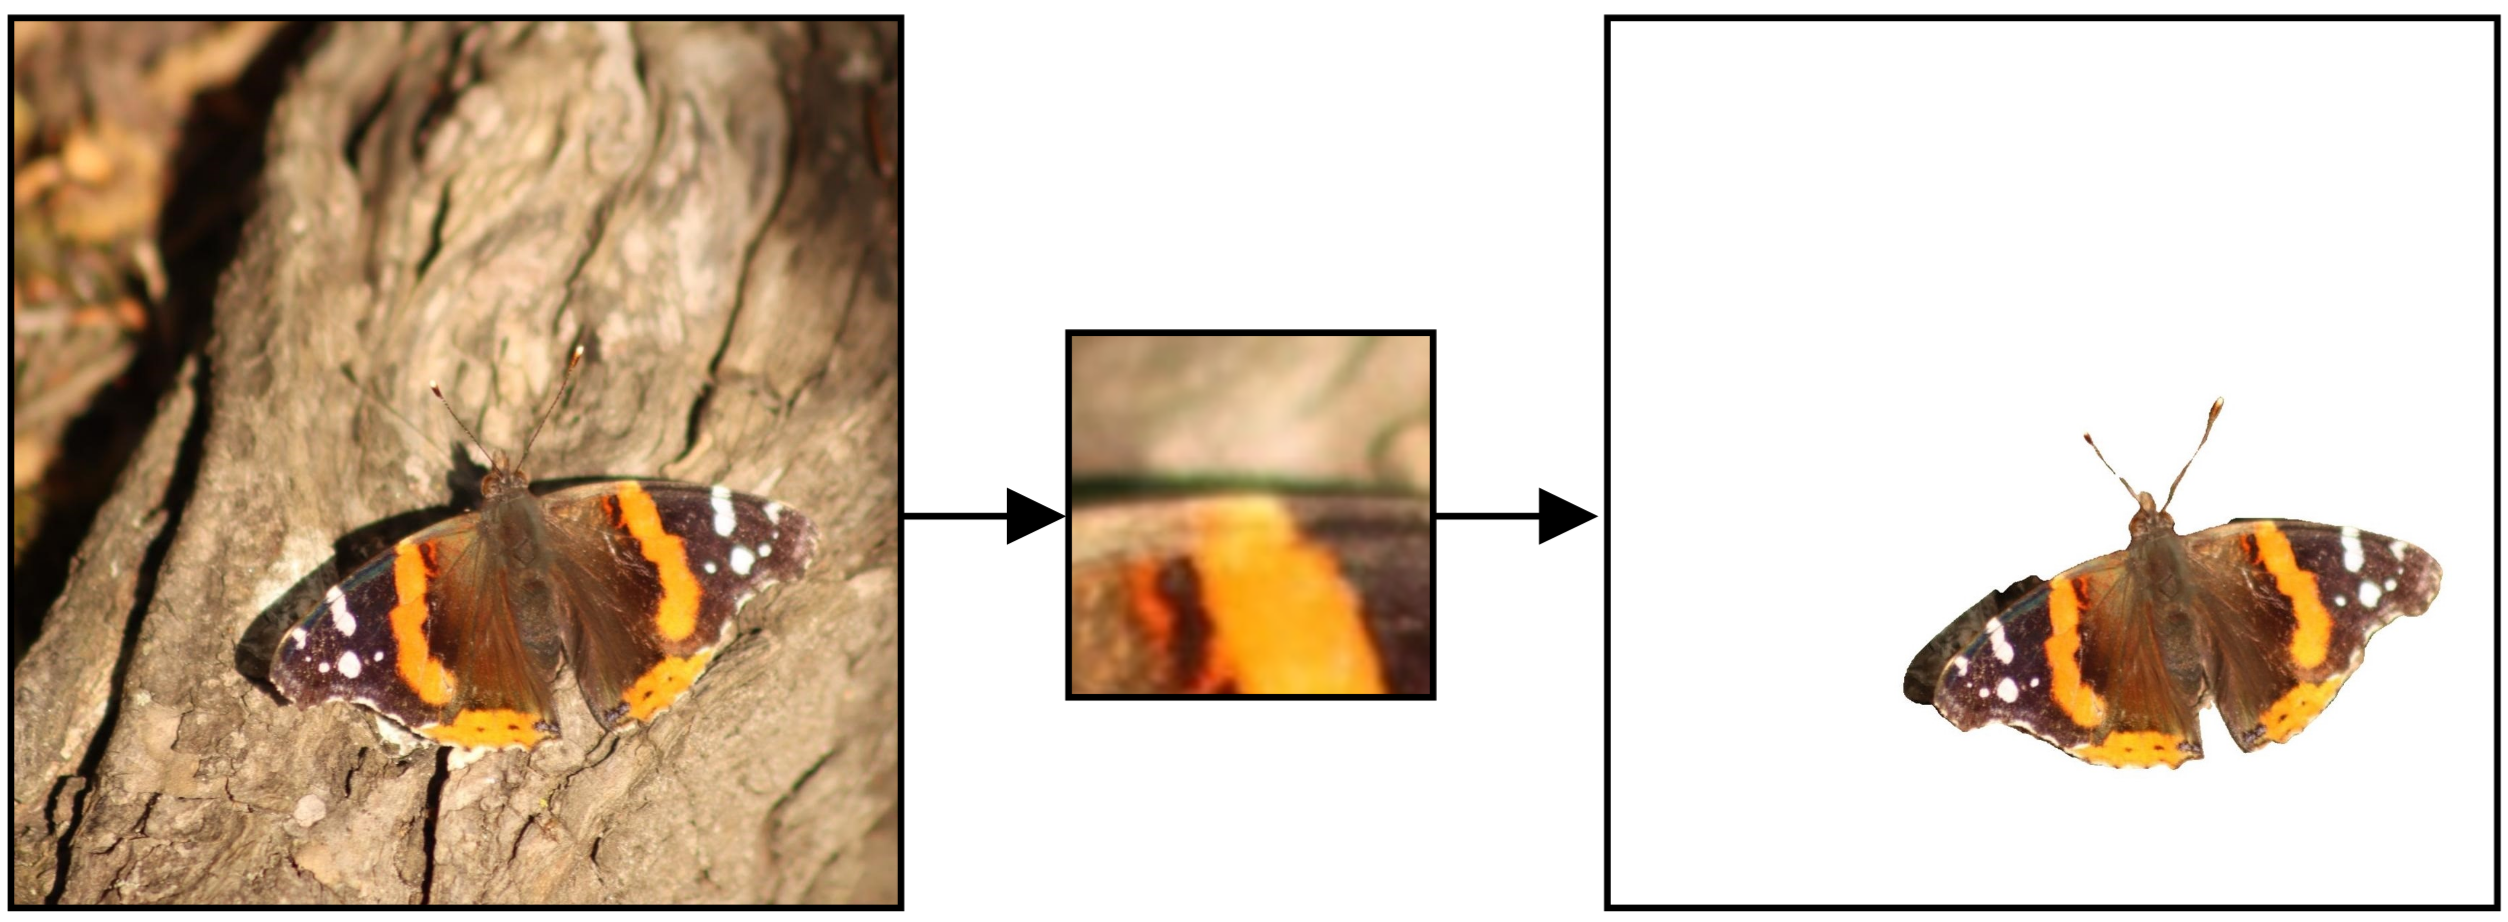
\includegraphics[width=.7\textwidth]{Sections/net/butterfly.png}
    \noindent\rule{\textwidth}{0.4pt}
    \caption{A high-level diagram of image segmentation.}
    \label{fig:butterfly}
    % Christian J. Rudder took this photo
\end{figure}

\noindent
We partition the image into two sets, via cut $C(A,B)$, $A$ the foreground and $B$ the background.
We the find a partition maximizing the likelihood of pixels in the foreground and background, while minimizing the penalties.
Hence, 
$$\displaystyle\max\left\{\sum_{i\in A} a_i + \sum_{j\in B} b_j - \sum_{(i,j)\in E} p_{ij}\right\}.$$

\noindent
However, we don't on hand have an algorithm to solve the maximum cut problem. We can however invert the max-cut into a min-cut problem.
\begin{theo}[Min-Max Inverse Function]

    Given a min function $f(x)$, the max function $-f(x)$ is equivalent to the min function $f(-x)$.
\end{theo}
We convert the previous function into the following min-cut problem: 
$\displaystyle\min\left\{-\sum a_i - \sum b_j + \sum p_{ij}\right\}.$ 
\textbf{Our Trick:} If we add a constant $C$ to our deciding function, the result is still the same, just shifted,
as all terms are still the same relative to each other. E.g., $\max\{x\} = \max\{x-C\}= \min\{-x+C\}= \min\{-x\}$, within a constant $C$.
We add back $\sum a_i + \sum b_j$ from the general set $V$ and group terms yielding:
$$\min\left\{\left(\sum_{j\in V} b_j - \sum_{i\in A} a_i \right) + \left(\sum_{i\in V} a_i - \sum_{j\in B} b_j\right) + \sum_{(i,j)\in E} p_{ij}\right\}=
\min\left\{\sum_{j\in B} a_j + \sum_{i\in A} b_i + \sum_{(i,j)\in E} p_{ij}\right\},$$
Giving us mis-labelings of $a$ and $b$ in $V$. Despite the inversion, it retains the same selection.

\newpage

\section*{Network Flow Setup}
We take $I(V,E)$ and convert it into a graph $G=(V,E)$, where each neighboring pixel $i$ and $j$ are connected by an edge $(i,j)$, with
$p_{ij}$ capacity. In the residual graph $G'$, we add two edges to represent flow from either $i\to j$ and $j\to i$.

\begin{Def}[Anti-parallel Edges]
    
    Given an edge $e$ and endpoints $i$ and $j$, the anti-parallel edges are $i\to j$ and $j\to i$, both 
    independent of each other.
\end{Def}

\vspace{-1em}
\begin{figure}[h]
    \centering
    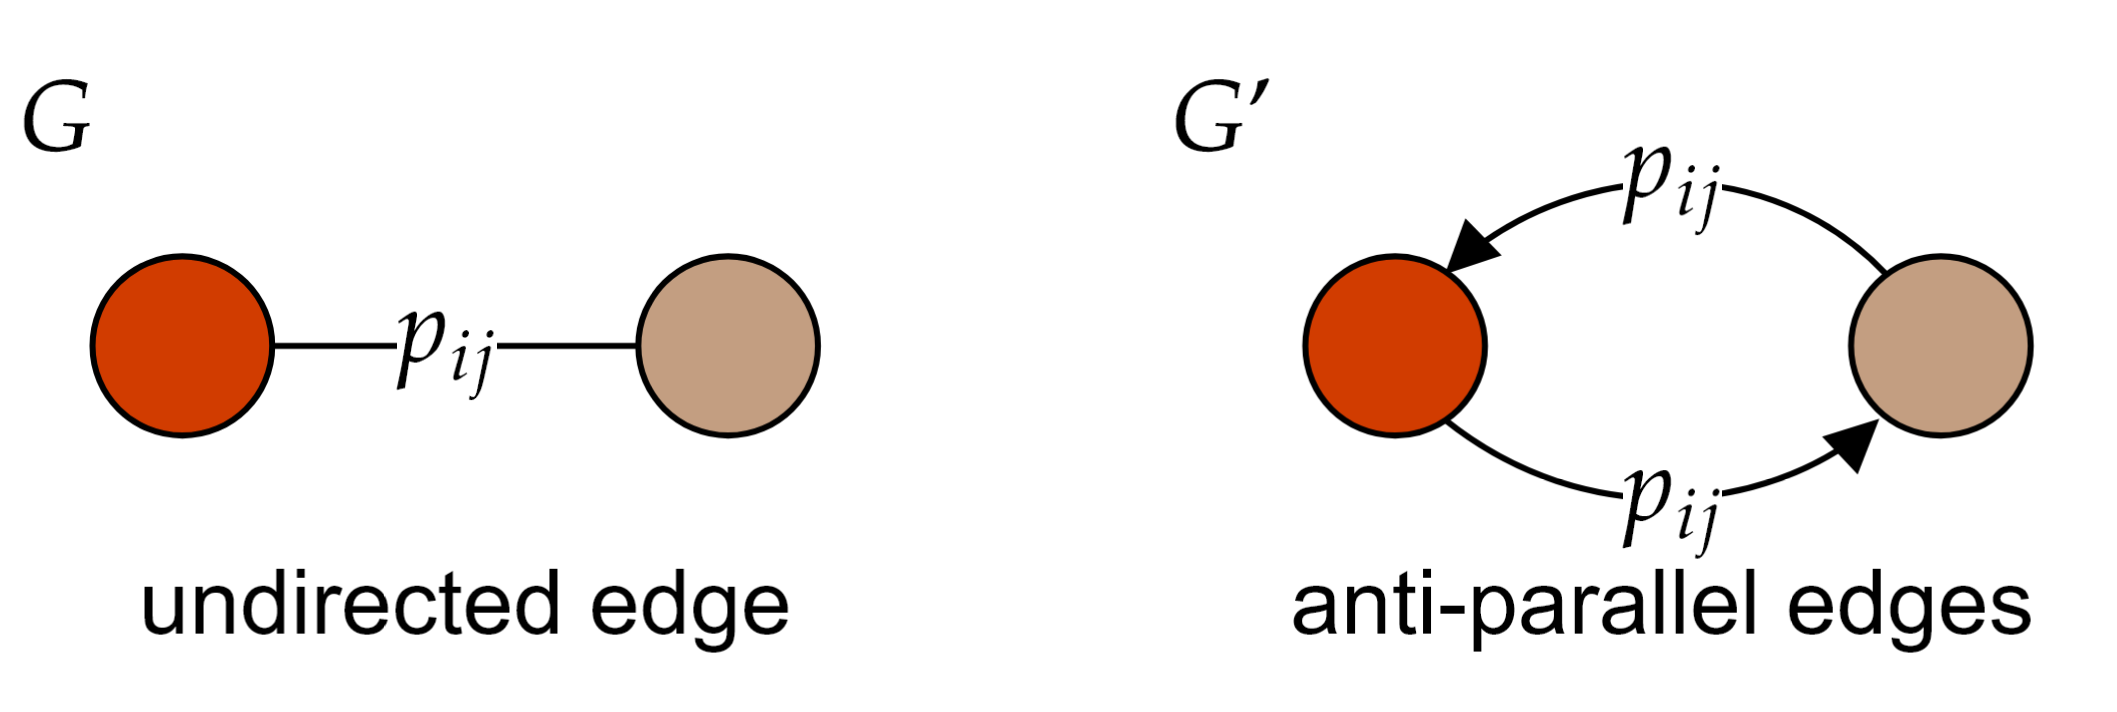
\includegraphics[width=.5\textwidth]{Sections/net/anti.png}
    \caption{Showing an edge in $G$ vs. its anti-parallel edges in $G'$.}
\end{figure}

\vspace{-1em}
\begin{Def}[Net-flow of Anti-parallel Edges]

    The net flow of the anti-parallel edges from a residual graph on endpoints $i$ and $j$ is given by,
    $$f(i,j) = f(i,j') - f(j,i').$$
\end{Def}
\noindent
This means the flow through endpoints $i$ and $j$ could be negative, zero, or positive. If negative, we have more flow from $j\to i$ than $i\to j$.
We now apply this to the Ford-Fulkerson algorithm.
\vspace{-1em}
\begin{figure}[h]
    \centering
    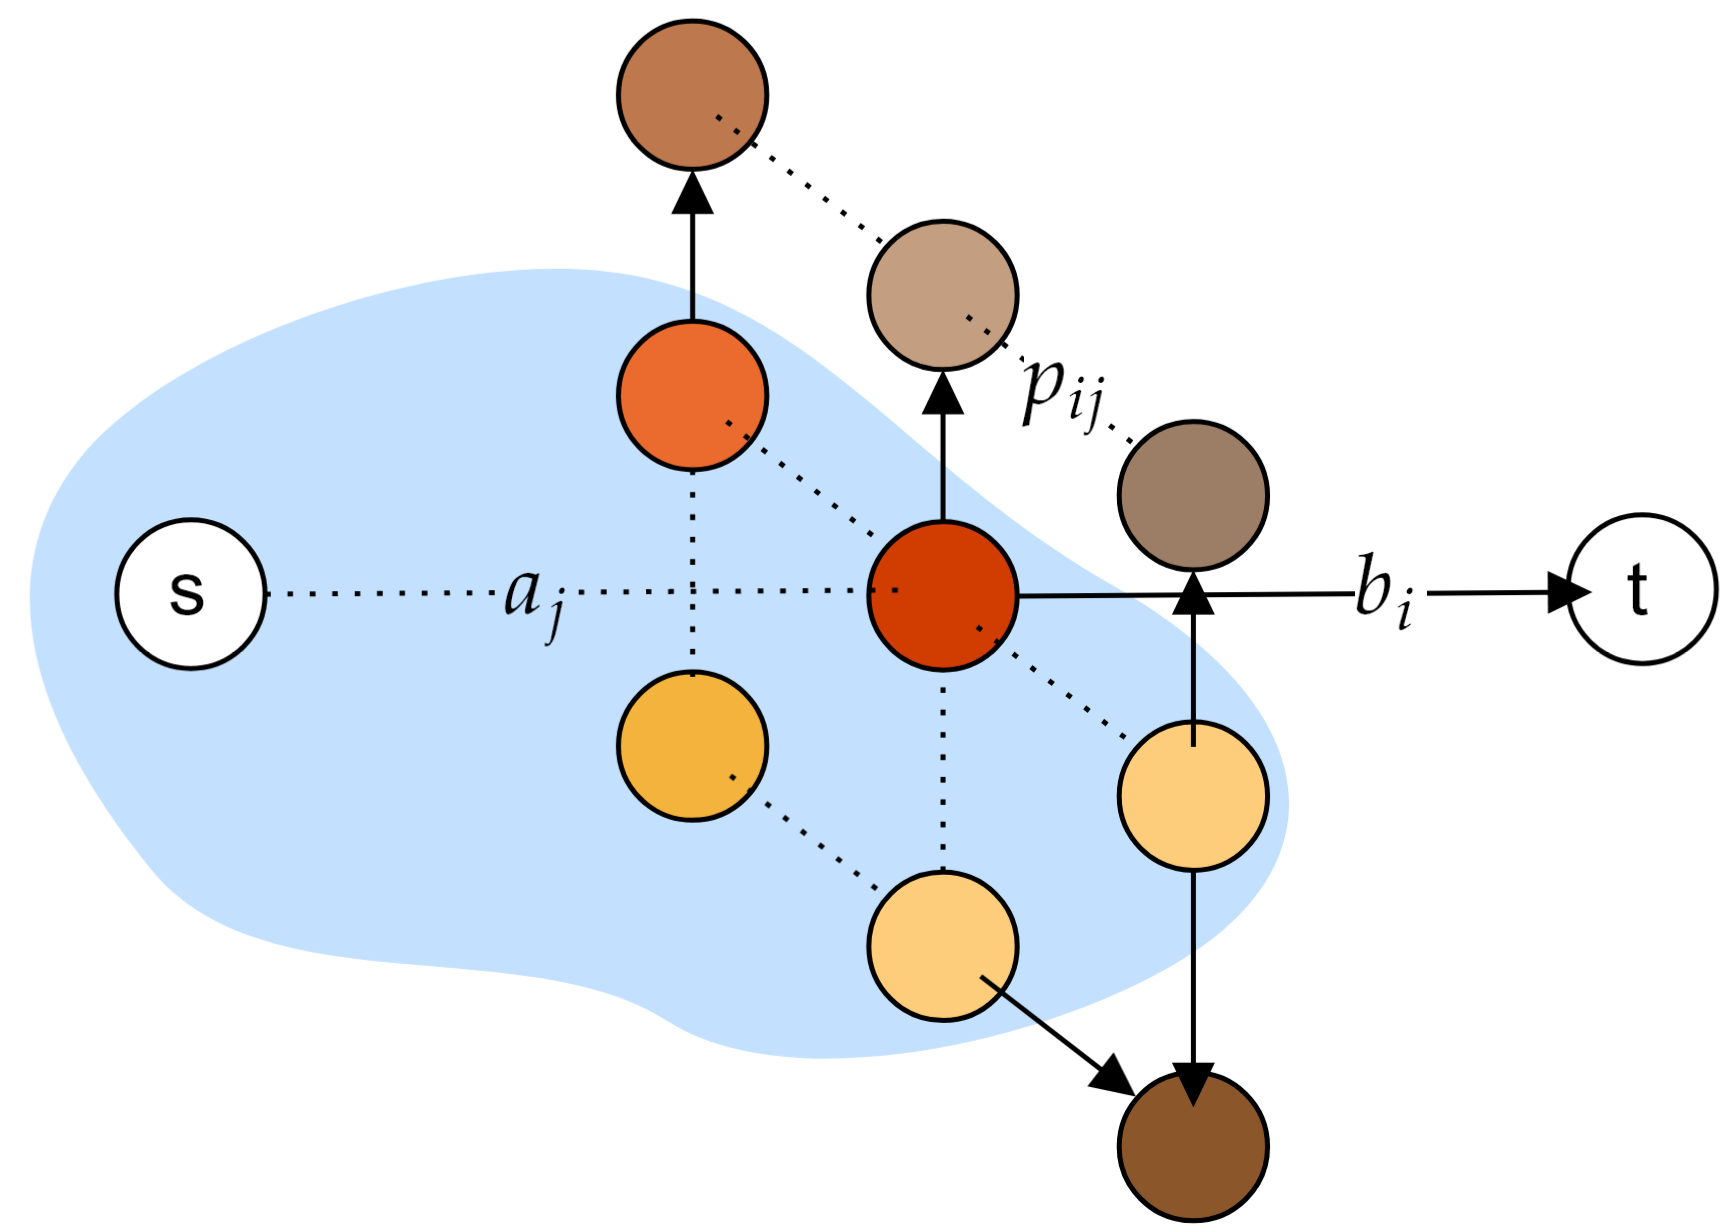
\includegraphics[width=.5\textwidth]{Sections/net/img.png}
    \caption{A flow network $G$ where the min-cut is highlighted in blue. Solid lines represent edges leaving the min-cut
    (not all connections from $s$ and $t$ to and from the image are shown).}
\end{figure}

\noindent
The derived min-cut yields the optimal partitioning of the image, separating foreground from background.





